\capitulo{4}{Conclusiones}

Desde pequeños hemos oído frases como ``Colócate bien la mochila que te vas a dañar la espalda'', ``Siéntate bien que dentro de unos años te va a doler la espalda'', ``Camina erguido''... Actualmente vivimos en un mundo muy heterogéneo y lleno de tecnologías, ¿por qué seguimos escuchando este tipo de frases? Es sencillo, porque no estamos acostumbrados a mantener una postura correcta. En eso se basa la idea que planteo, en crear un dispositivo que nos ayude a acostumbrarnos a una postura correcta para disminuir daños, además de ayudar a distintos grupos de personas con ciertas patologías que les impide mantener una postura correcta o que se olvidan de mantenerse correctamente erguidos, patologías como puede ser el Parkinson. 

En este trabajo se han estudiado las bases de la postura y del control postural y su constante modificación a lo largo de la vida de una persona. Asimismo, se han conocido algunas de las opciones que existen en la actualidad para controlar o monitorizar la postura de un usuario, incluyendo algunos dispositivos de diagnóstico de alteraciones posturales y algunos estudios realizados respecto al desarrollo de dispositivos posturales.

Finalmente, gracias a los conocimientos adquiridos durante la búsqueda de información para el proyecto y los adquiridos a lo largo de la titulación, se han conseguido dos prototipos sencillos basados en una tecnología de código abierto, Arduino, que permiten mejorar la postura empleando el aprendizaje dinámico basado en biofeedback. 

Como complemento del proyecto se ha ideado un prototipo de interfaz en el que se aúnan las características principales de las aplicaciones existentes de los dispositivos de control postural actuales.


\section{Resumen de resultados.}

Como se ha mencionado previamente, se han creado dos prototipos de un dispositivo de control postural. La primera versión del prototipo es la más sencilla, se ha empleado un sensor de inclinación SW520D que actúa como un interruptor. Mientras la persona se encuentre en una buena postura, se considerará como apagado y cuando la persona se inclina hacia delante, el dispositivo alertará a modo de biofeedback sonoro o vibratorio para que la persona recupere su postura correcta. 

Adicionalmente el primer prototipo incluye un botón de encendido, un led que indica que el dispositivo se encuentra encendido, un zumbador pasivo que emitirá la señal sonora para avisar al usuario y un motor de vibración que emitirá una señal vibratoria. Aunque, este último componente no se ha podido conseguir para la demostración. Se pueden ver imágenes del primer prototipo en las figuras \textit{Figura \ref{fig:imgDispositivo_V1}} y \textit{Figura \ref{fig:imgDispositivo_V1_sensor}}.

\begin{figure}[h!]
    \centering
    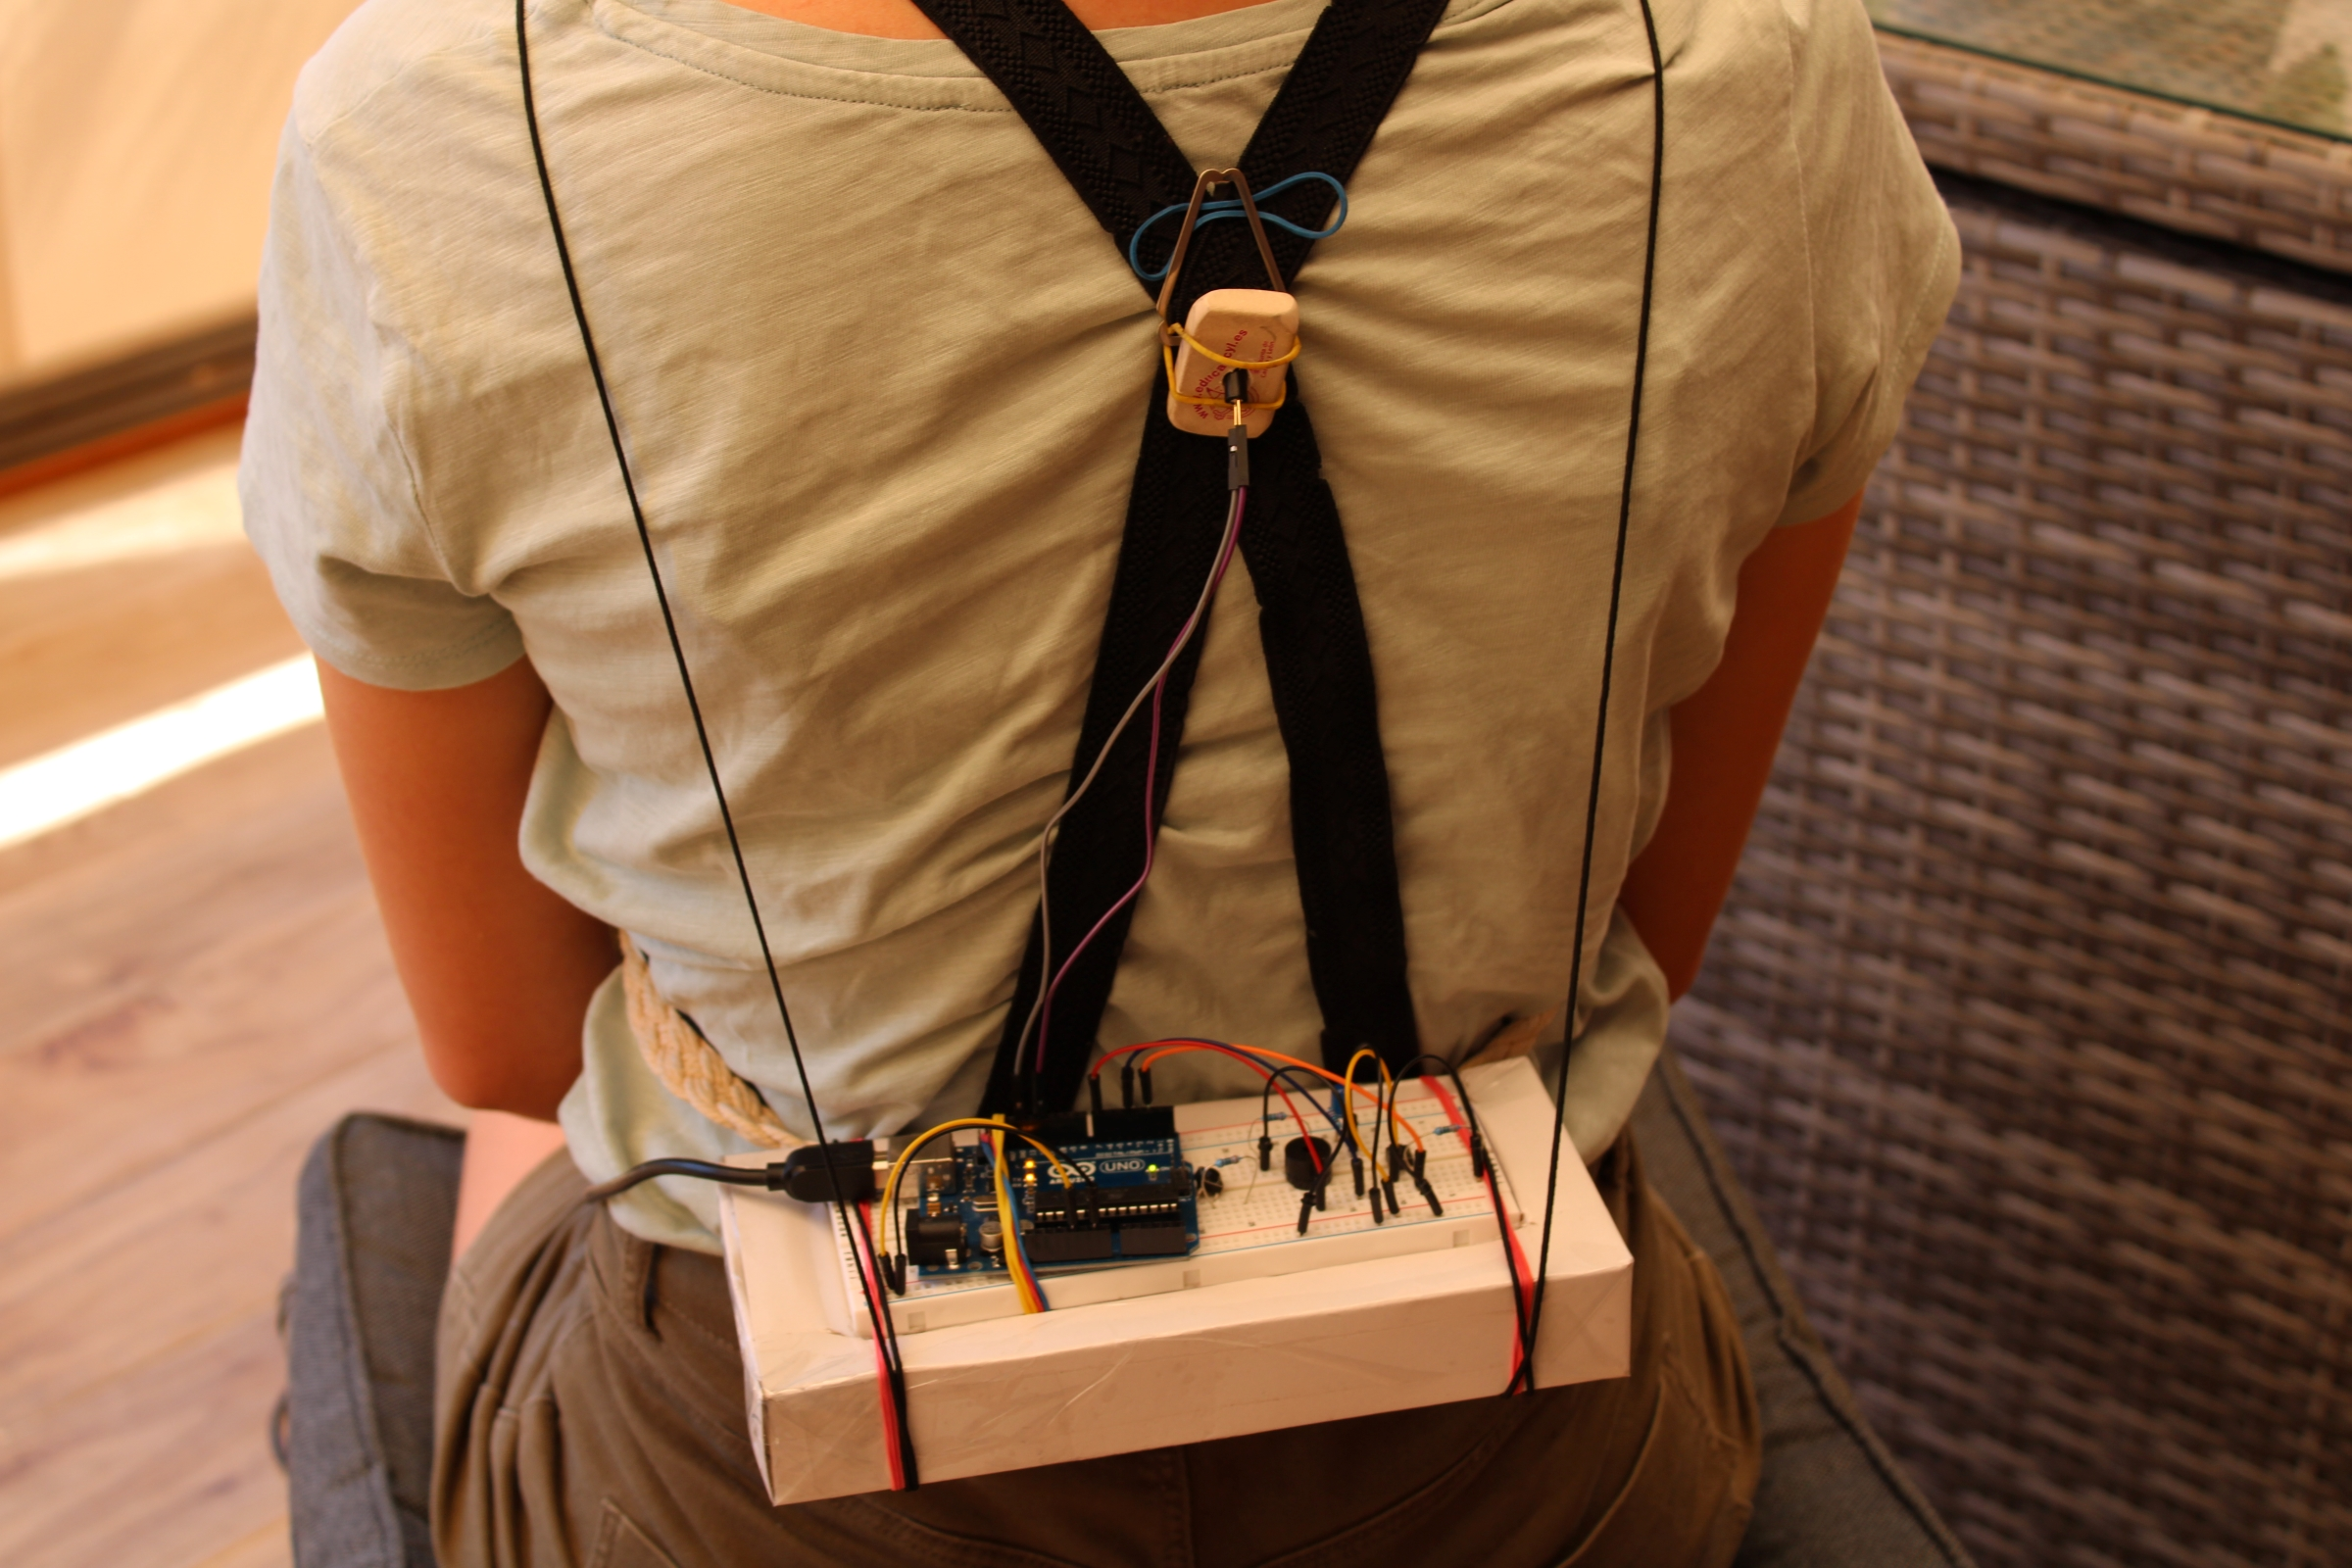
\includegraphics[width=0.5\textwidth]{img/Disp_V1_1.jpg}
    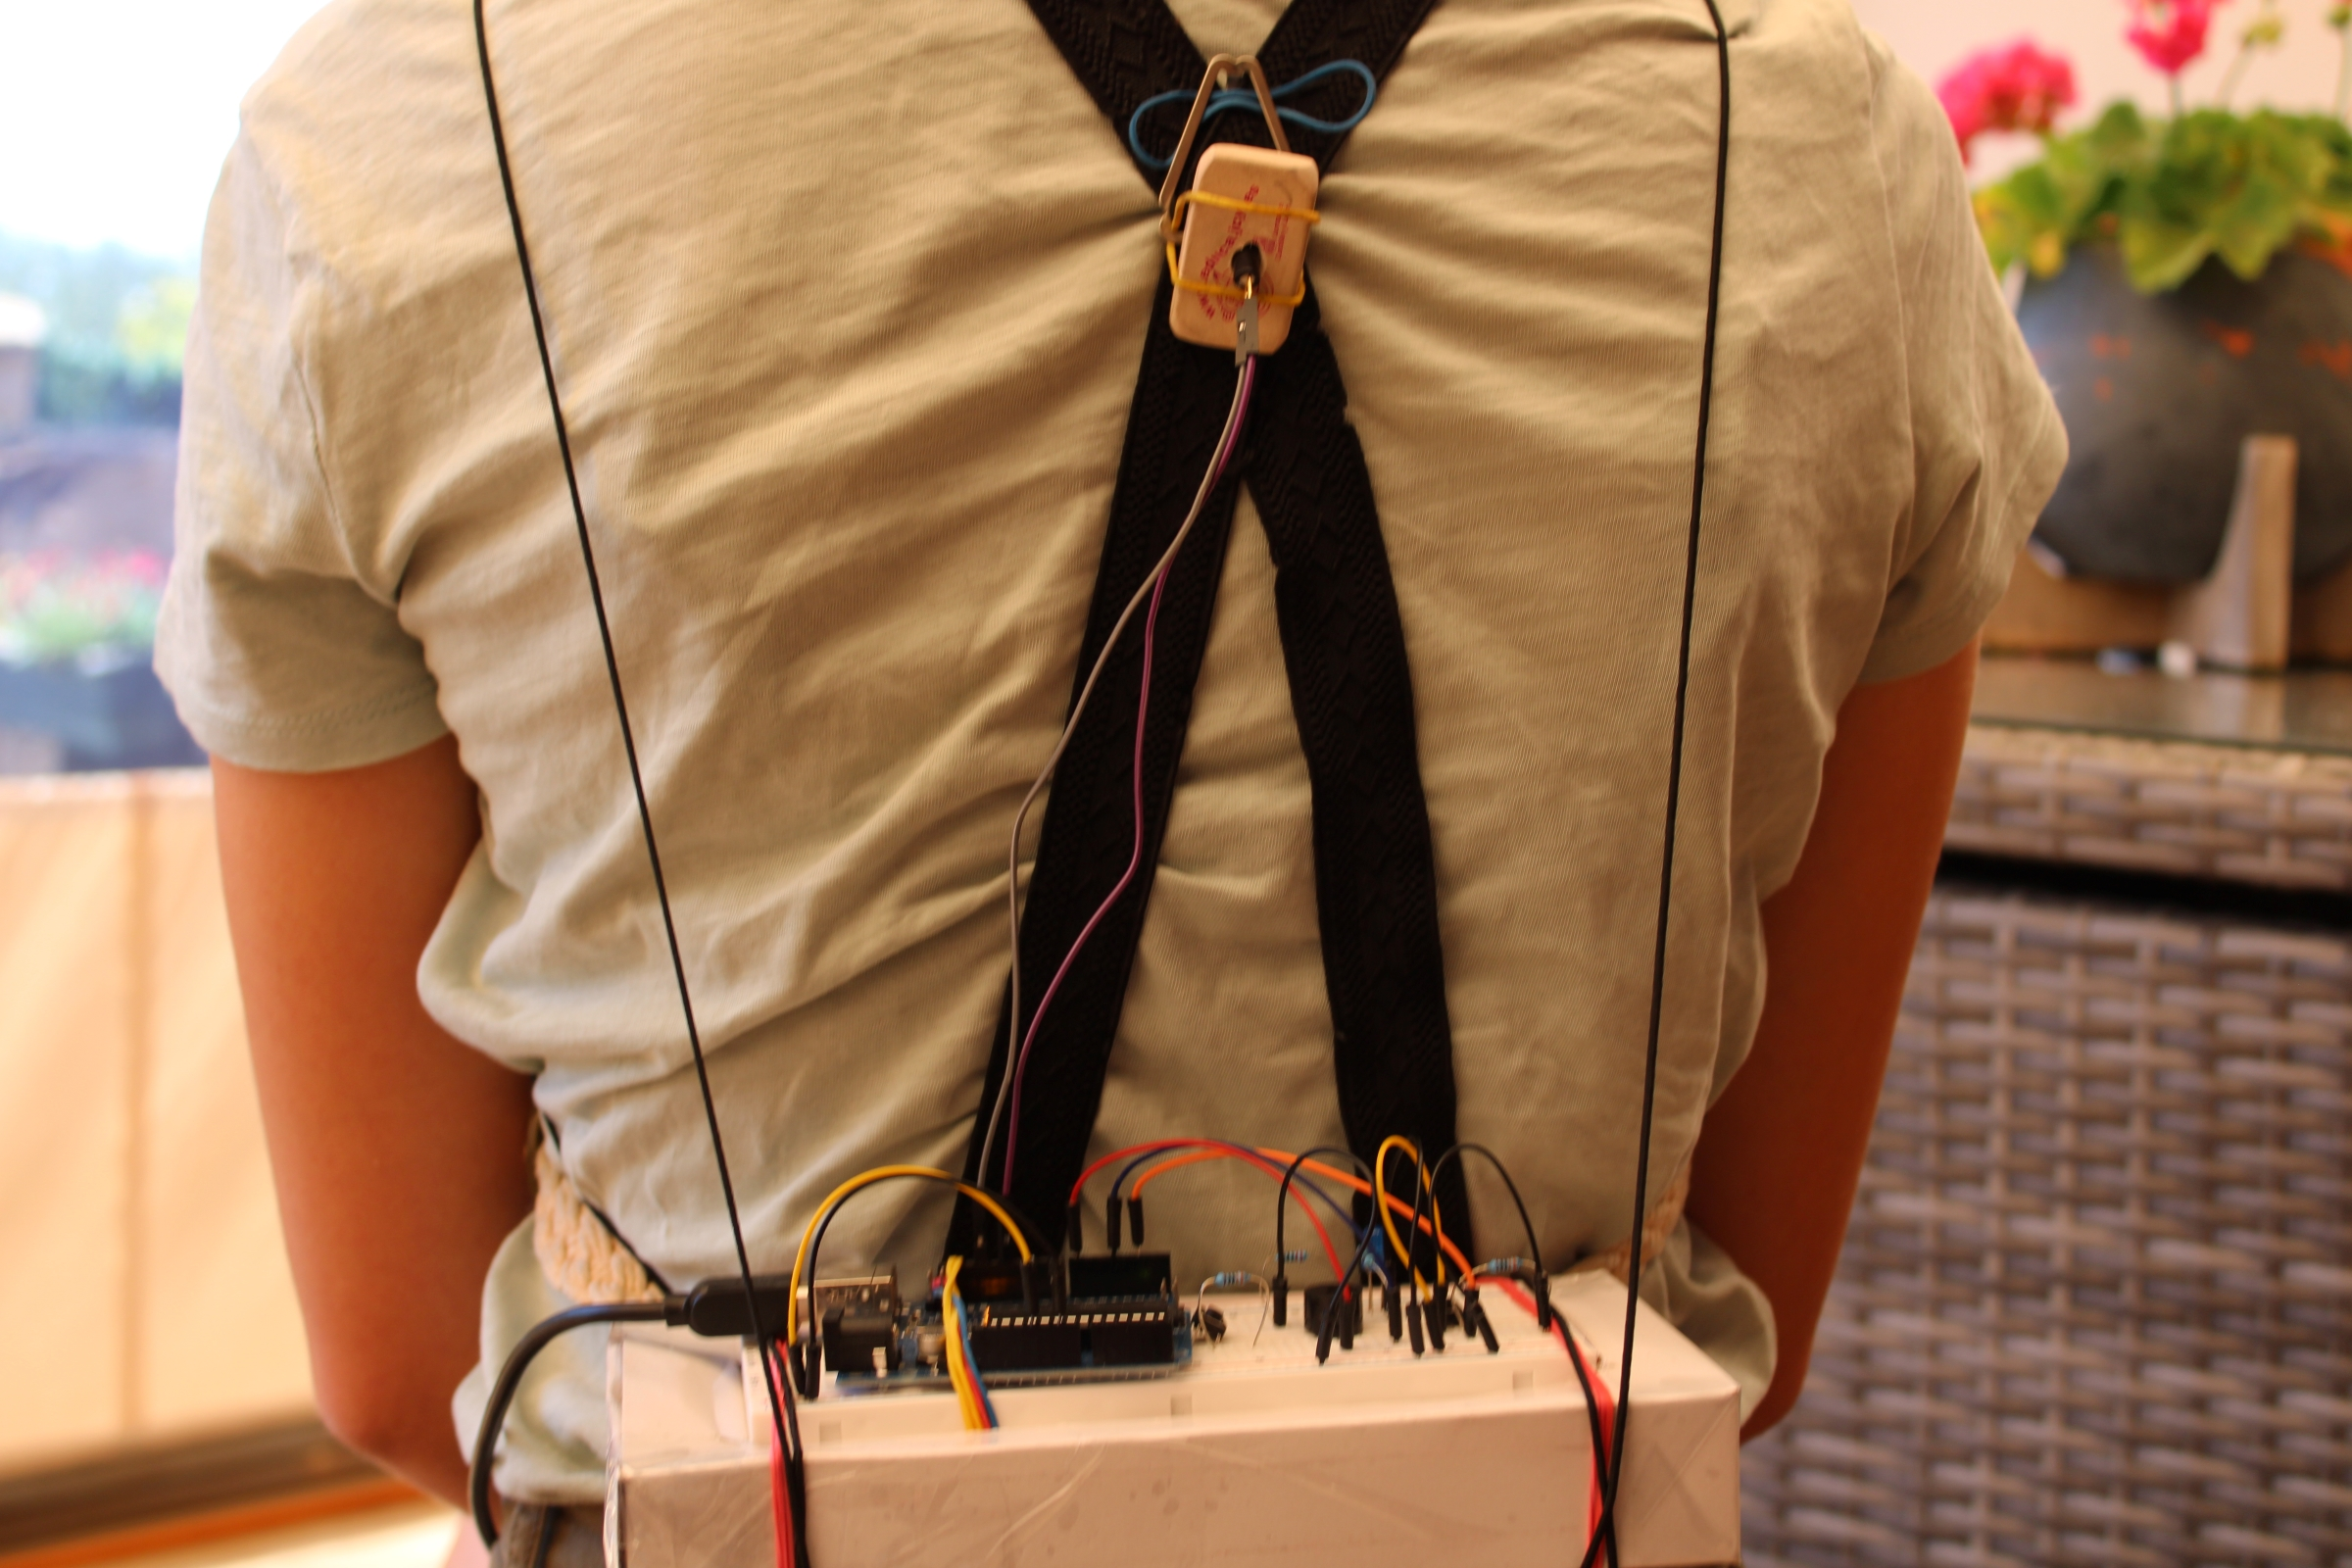
\includegraphics[width=0.5\textwidth]{img/Disp_V1_2.jpg}
    \caption{Imágenes del primer prototipo. Fuente Propia.}
    \label{fig:imgDispositivo_V1} 
\end{figure}

\begin{figure}[h!]
    \centering
    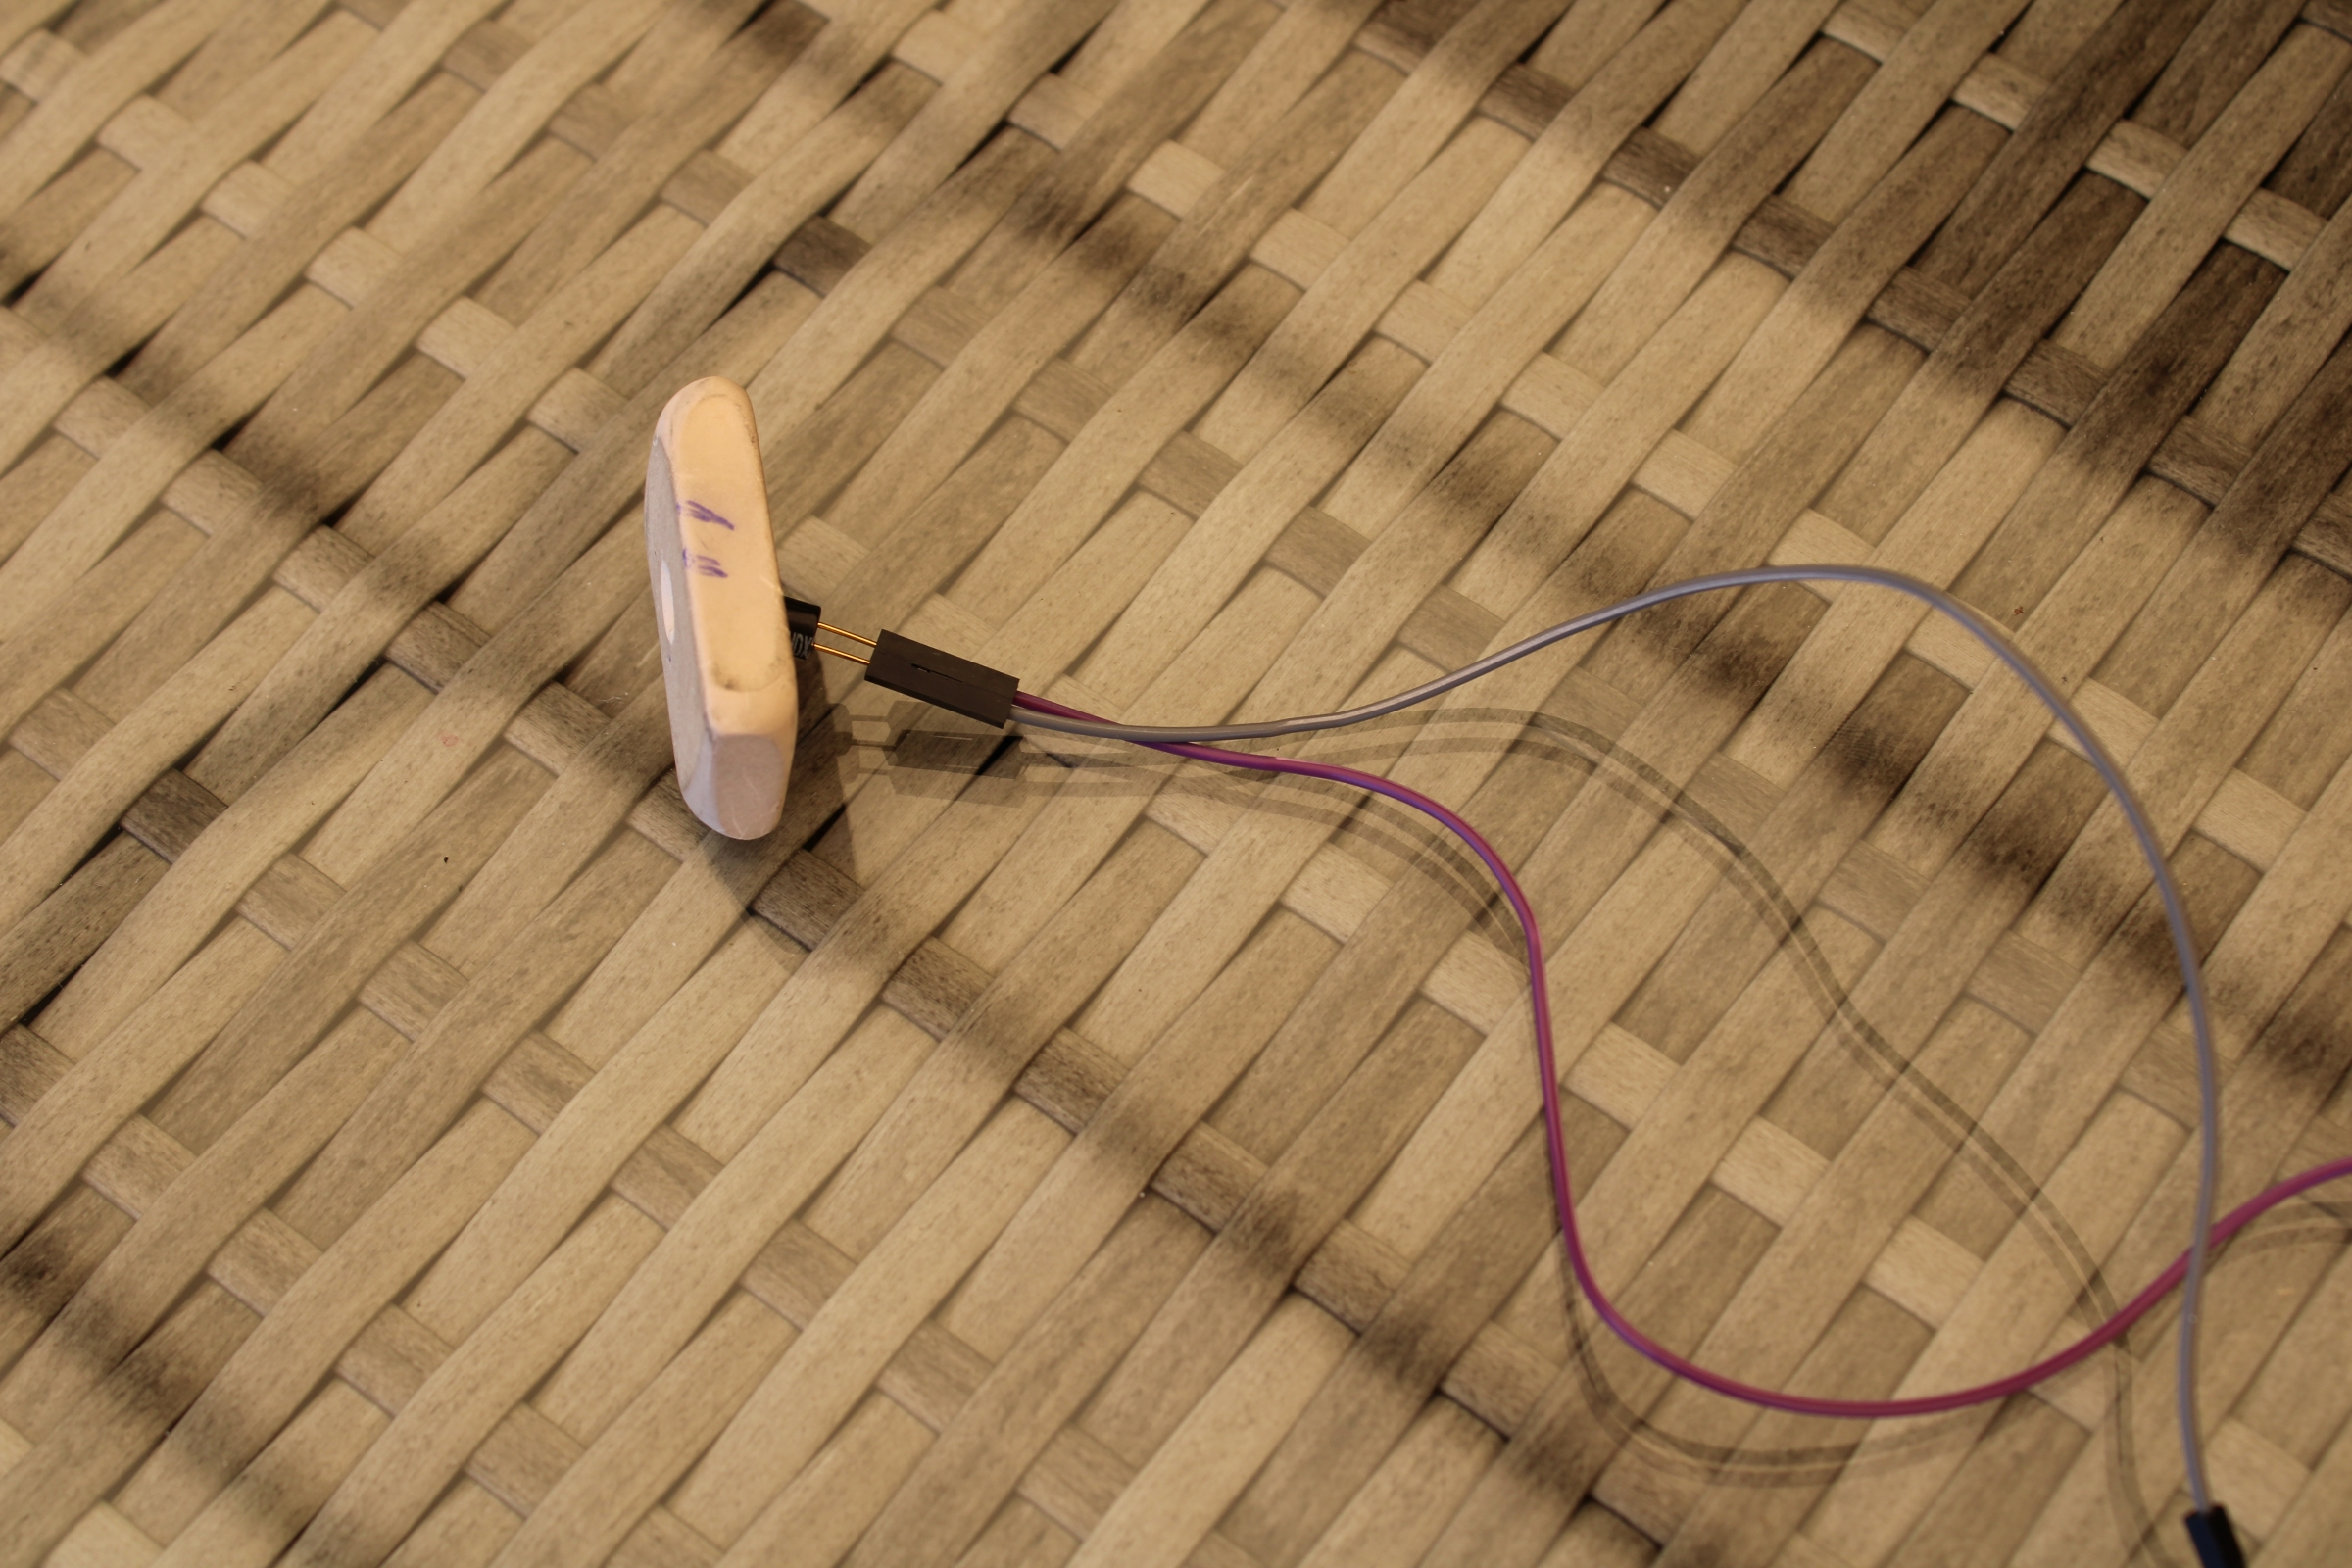
\includegraphics[width=0.4\textwidth]{img/SensorV1_1.jpg}
    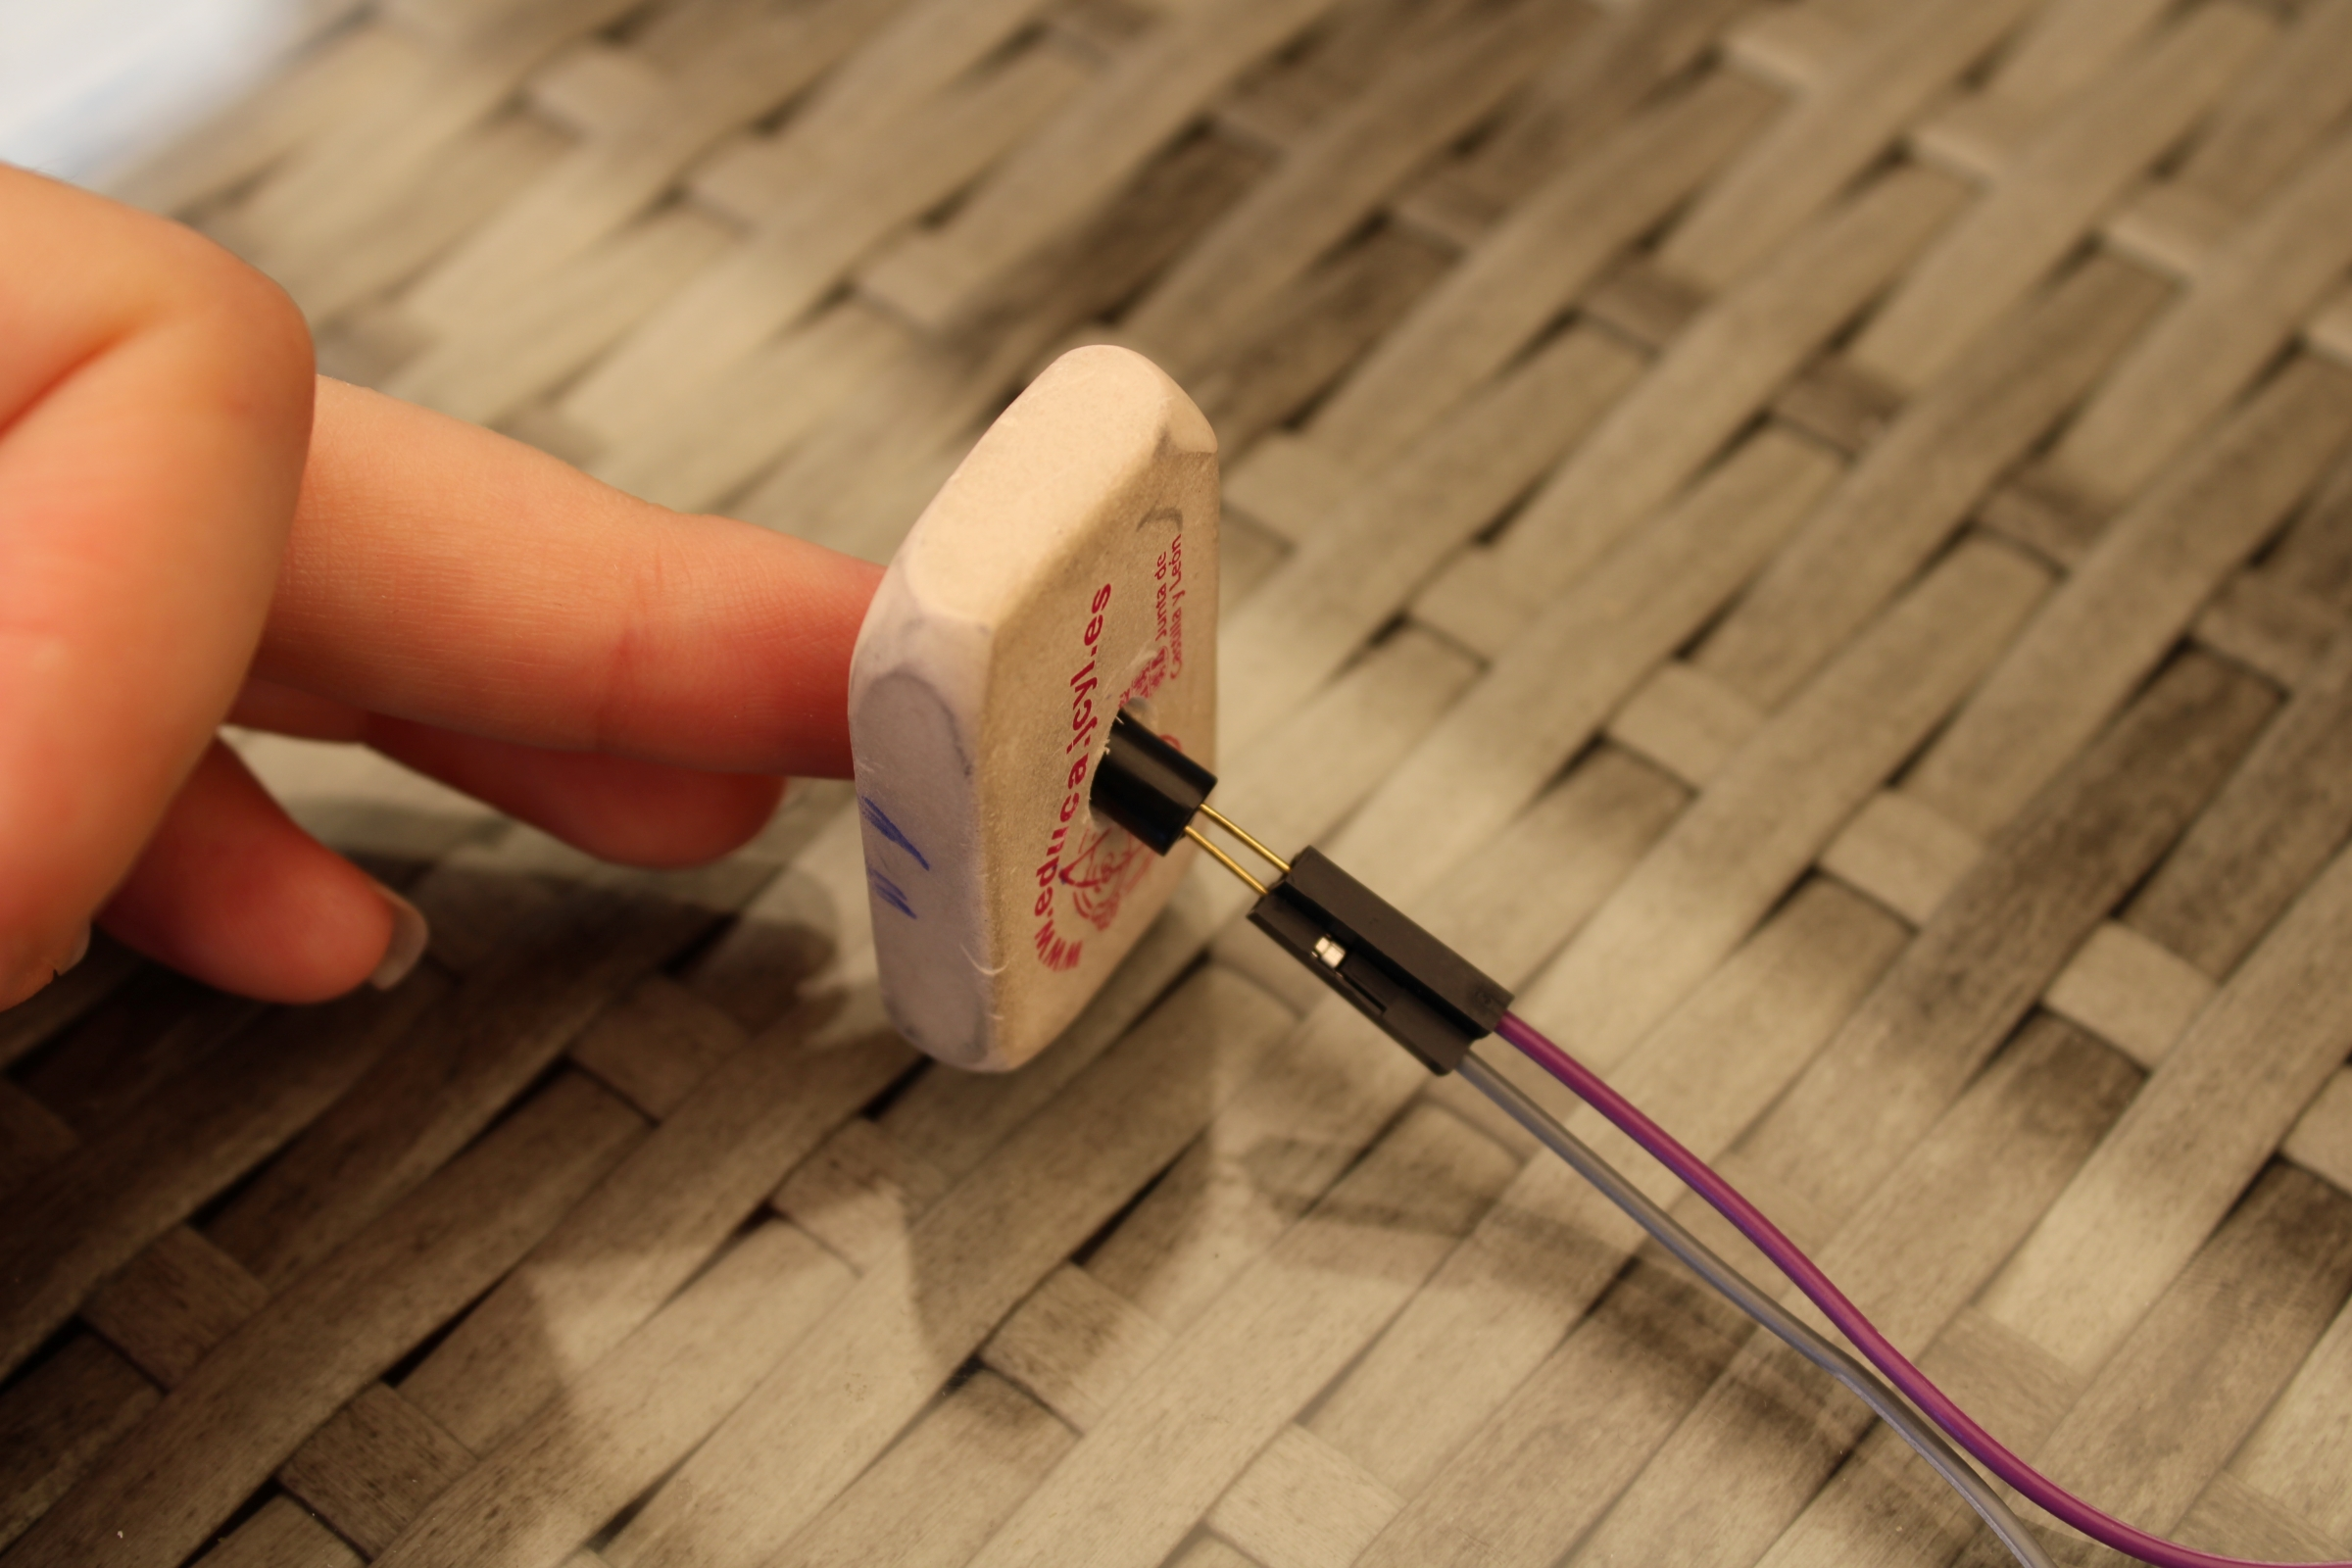
\includegraphics[width=0.4\textwidth]{img/SensorV1_2.jpg}
    \caption{Imágenes del sensor y su base  primer prototipo. Fuente Propia.}
    \label{fig:imgDispositivo_V1_sensor} 
\end{figure}

El sensor empleado en la primera versión es muy sensible a vibraciones y por ello se estudiaron otras posibilidades y se realizó un segundo prototipo.

La segunda versión consta de los mismos componentes que la primera versión integrando un botón de calibración y modificando el sensor SW520D\cite{SW520D_1} a un sensor más complejo, el MPU-6050\cite{MPU6050_1,MPU6050_2}, que permite una solución más precisa y amplia, midiendo aceleraciones y rotaciones en los ejes \textit{x},\textit{y} y \textit{z}. El hecho de medir las aceleraciones nos permite calcular por triangulación los ángulos de inclinación. Estos ángulos de inclinación son los que han sido empleados para diferenciar entre una buena o una mala postura, si se supera el ángulo umbral, se considerará como un postura incorrecta y si se mantiene dentro del umbral, se considerará una postura correcta. Al igual que en la primera fase si se detecta una mala postura se avisará al usuario mediante biofeedback sonoro o vibratorio. De igual modo, este sensor permitiría no solo cumplir con la función de control postural a la vez que garantiza la obtención de datos que se pueden emplear para la realización de estadísticas. Se pueden ver imágenes de esta segunda versión del prototipo en las figuras \textit{Figura \ref{fig:imgDispositivo_V2}} y \textit{Figura \ref{fig:imgDispositivo_V2_sensor}}.

\begin{figure}[h!]
    \centering
    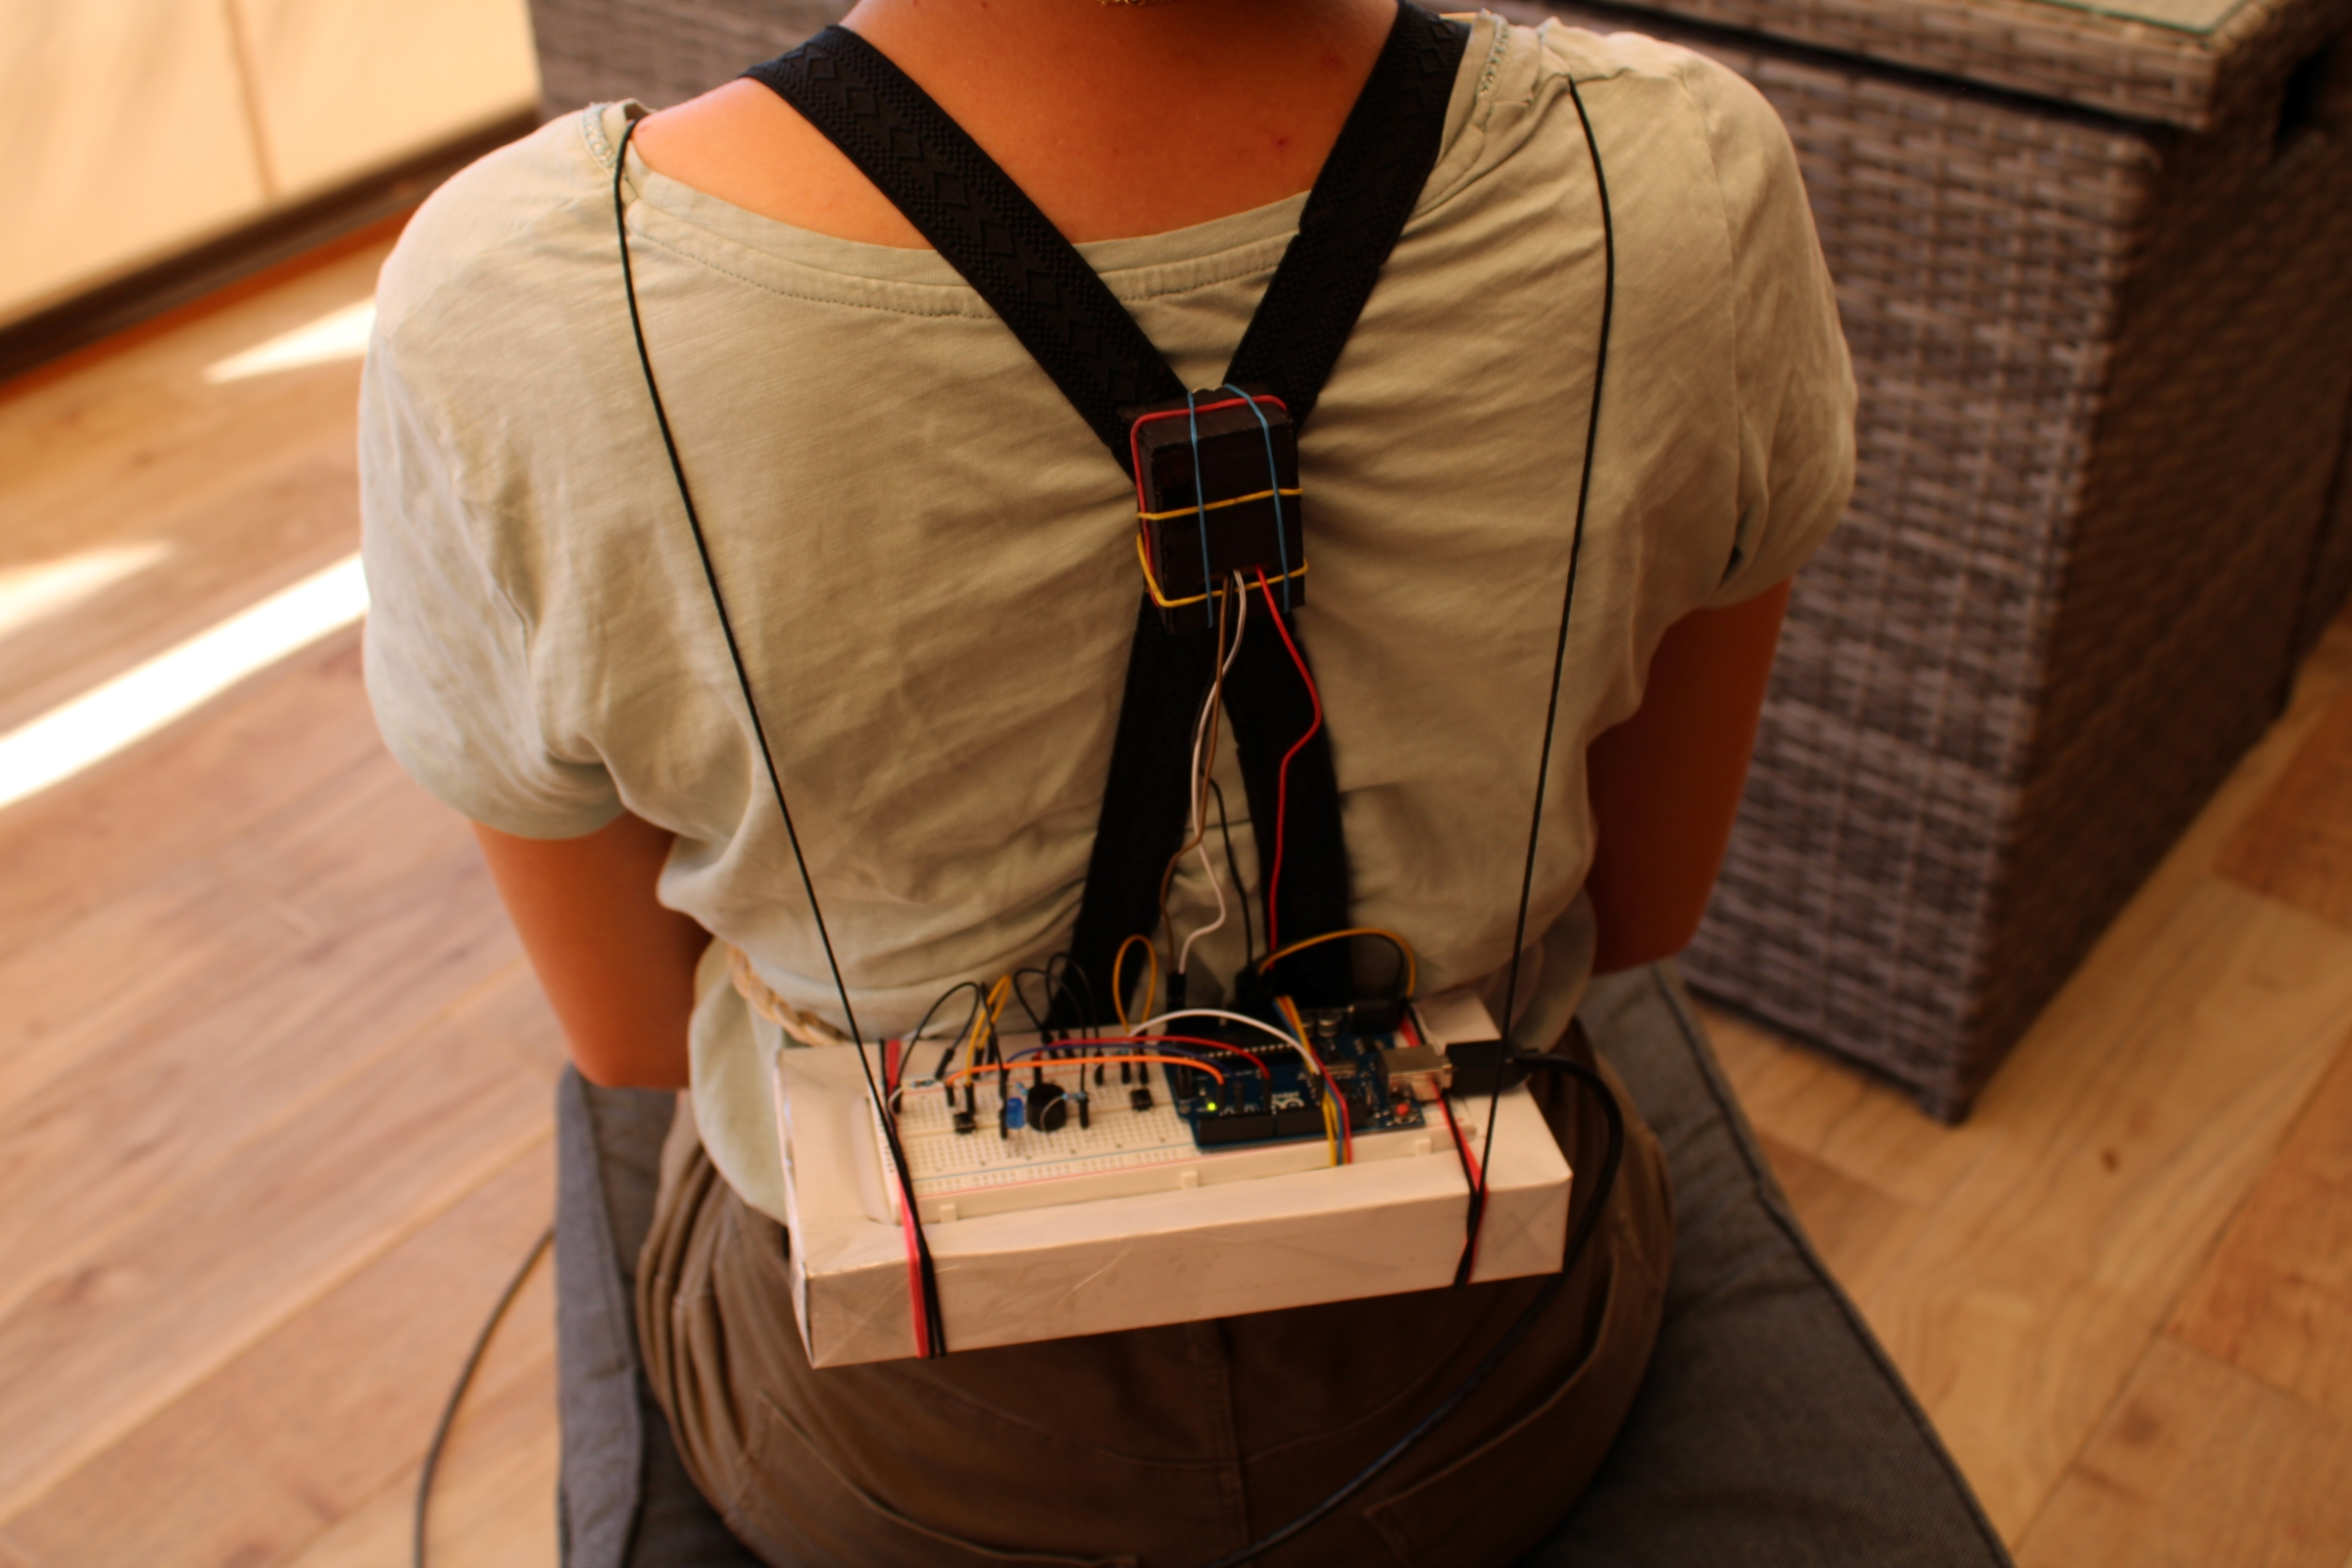
\includegraphics[width=0.4\textwidth]{img/Disp_V2_1.jpg}
    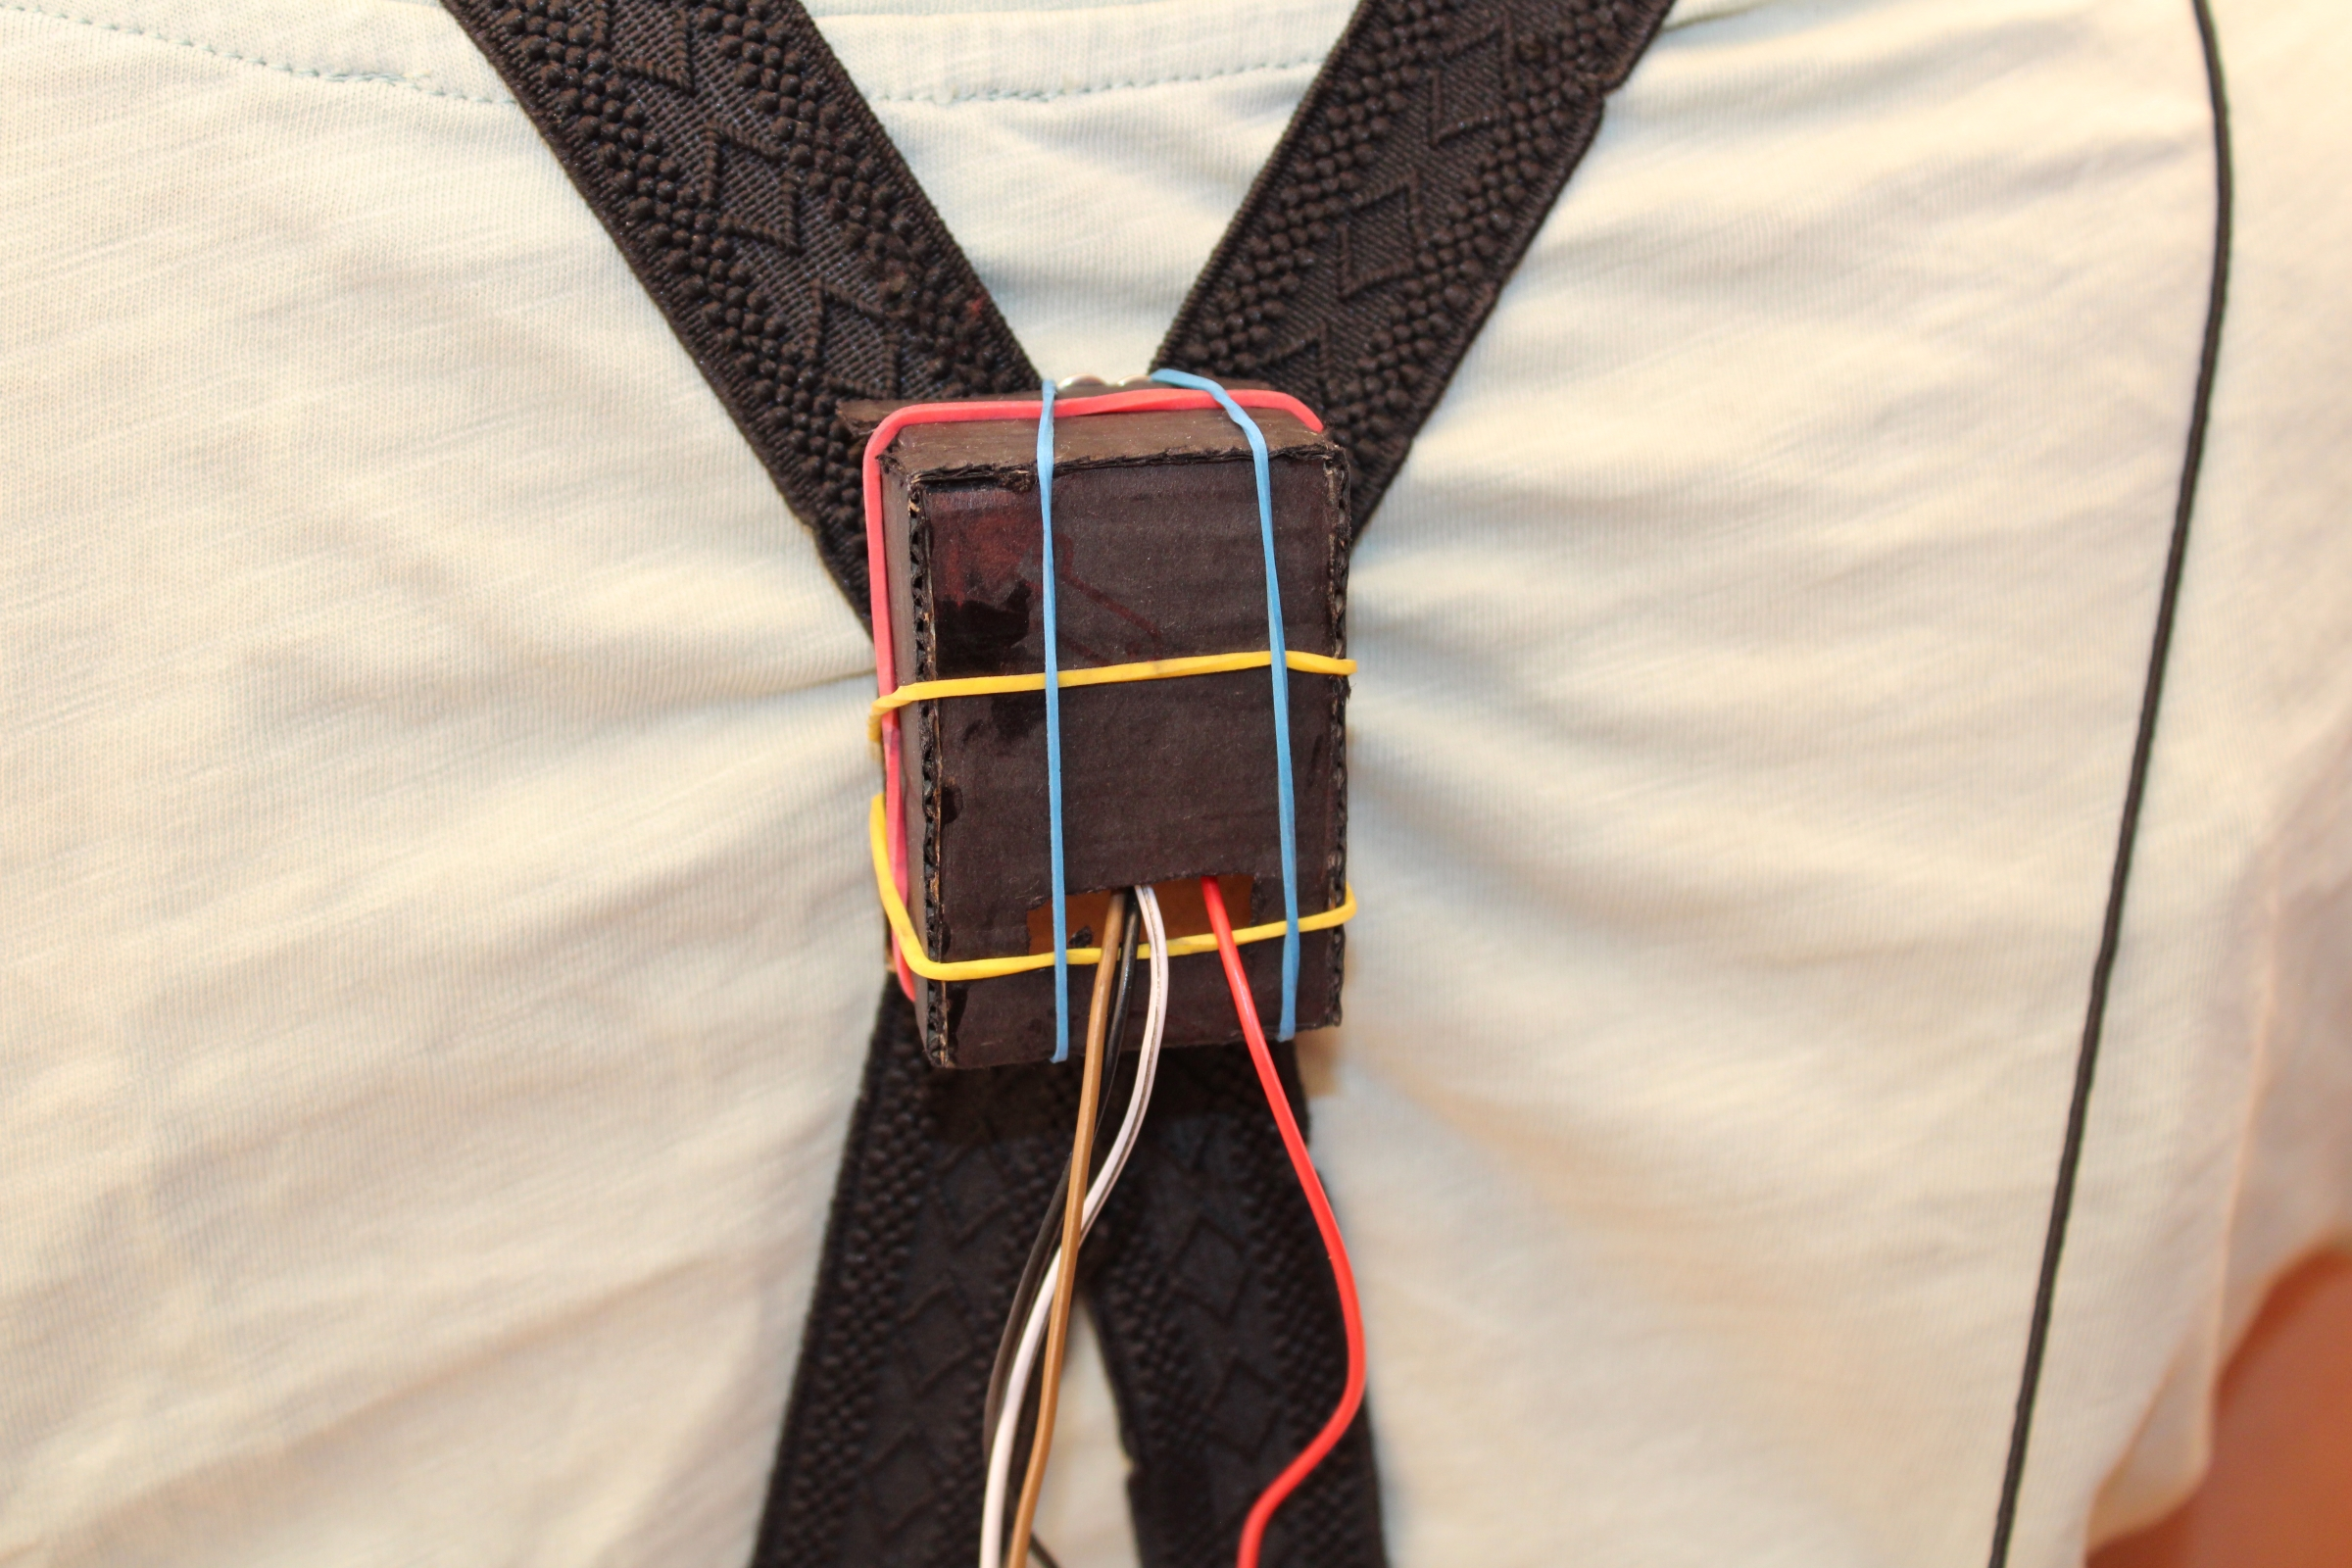
\includegraphics[width=0.4\textwidth]{img/Disp_V2_2.jpg}
    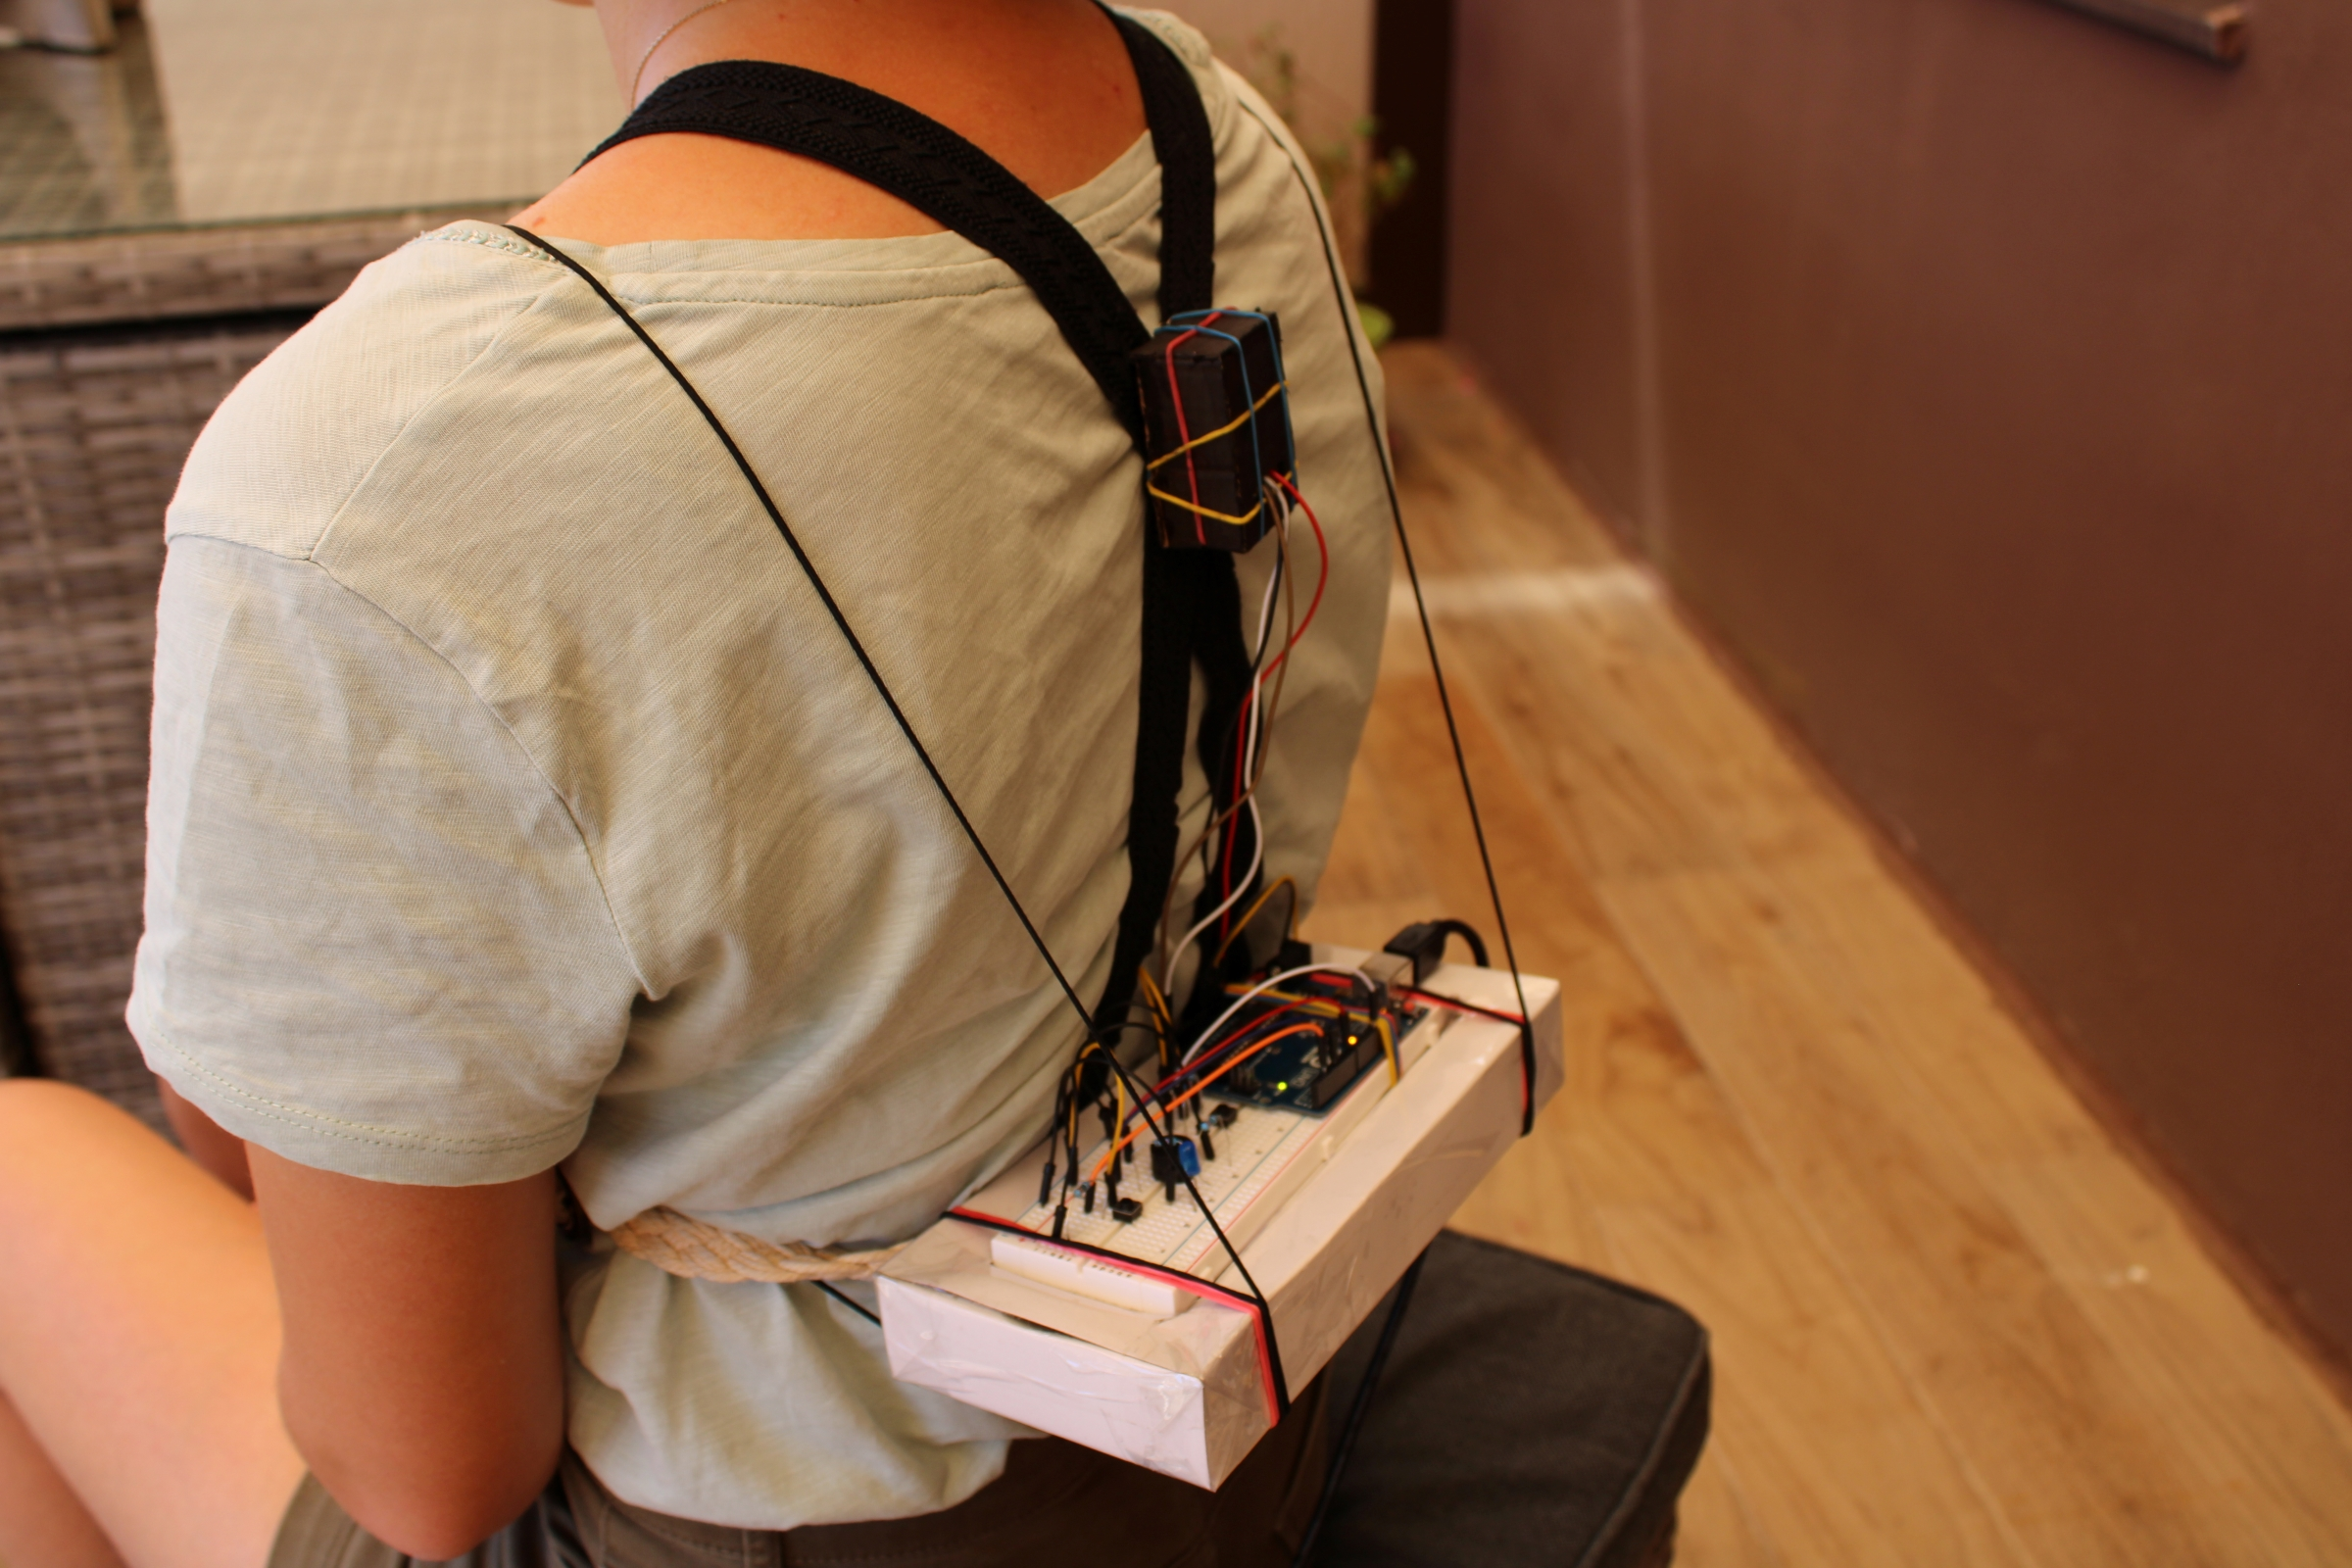
\includegraphics[width=0.4\textwidth]{img/Disp_V2_3.jpg}
    \caption{Imágenes de la segunda versión del prototipo. Fuente Propia.}
    \label{fig:imgDispositivo_V2} 
\end{figure}

\begin{figure}[h!]
    \centering
    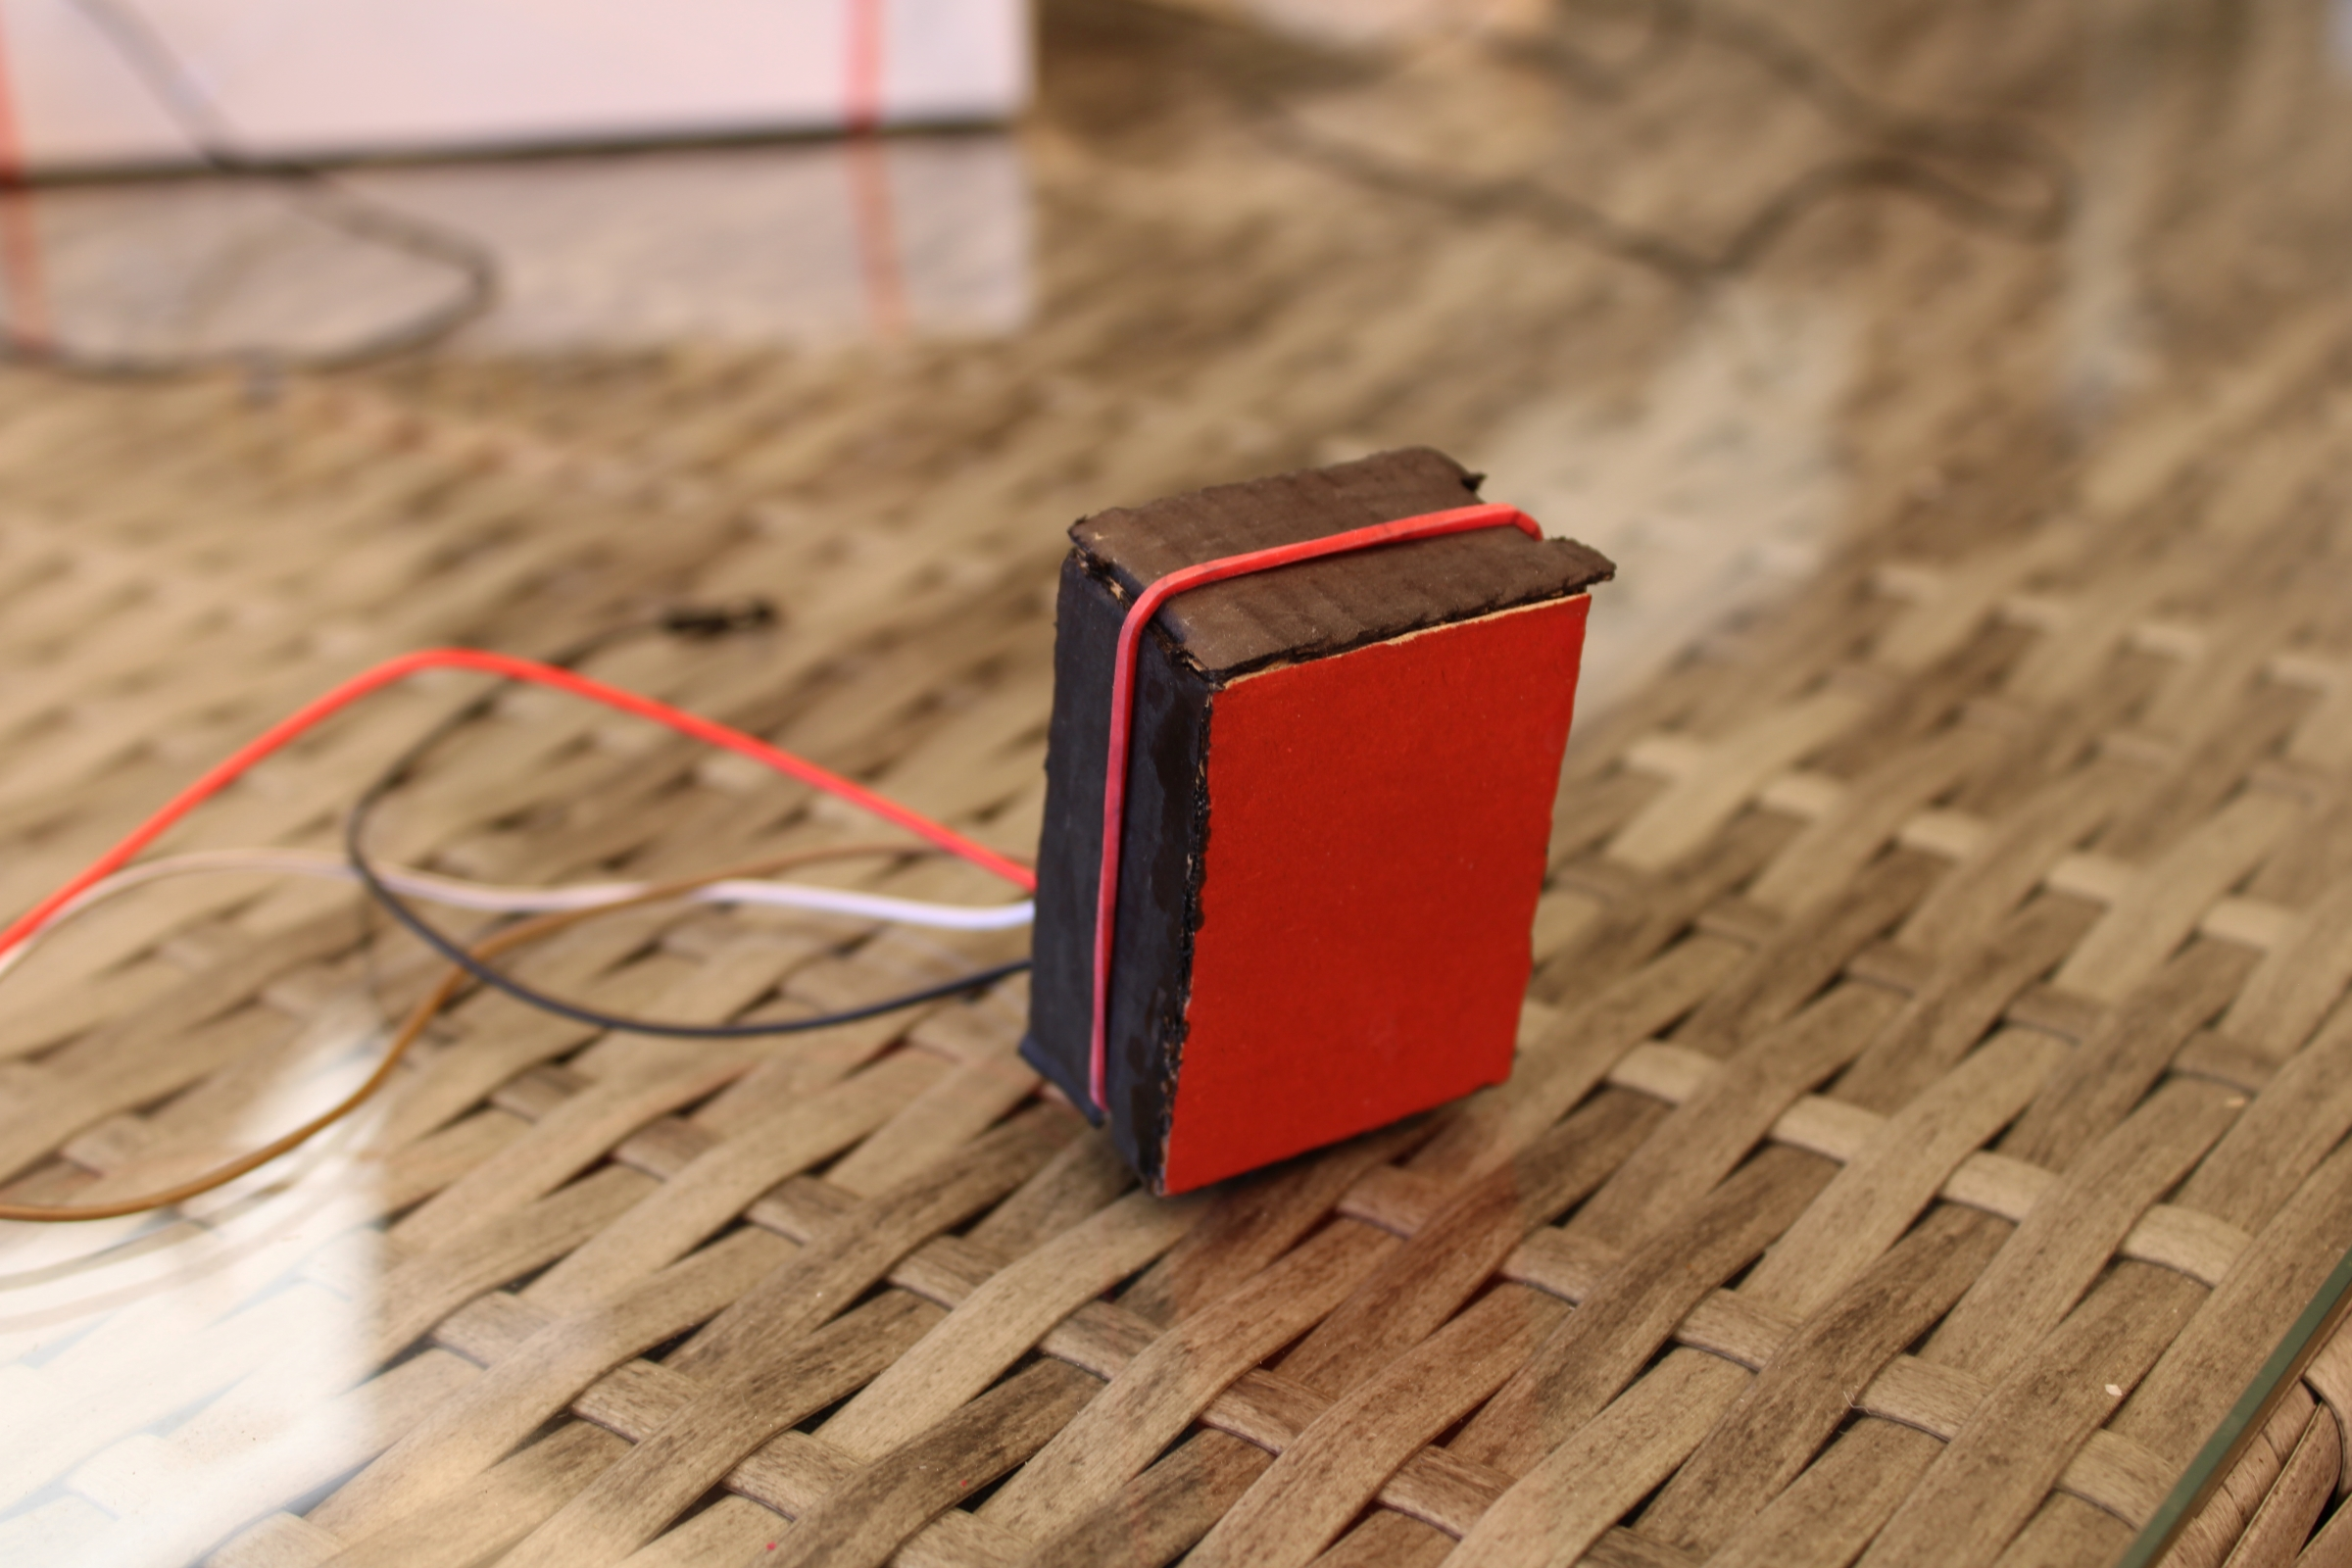
\includegraphics[width=0.4\textwidth]{img/SensorV2_1.jpg}
    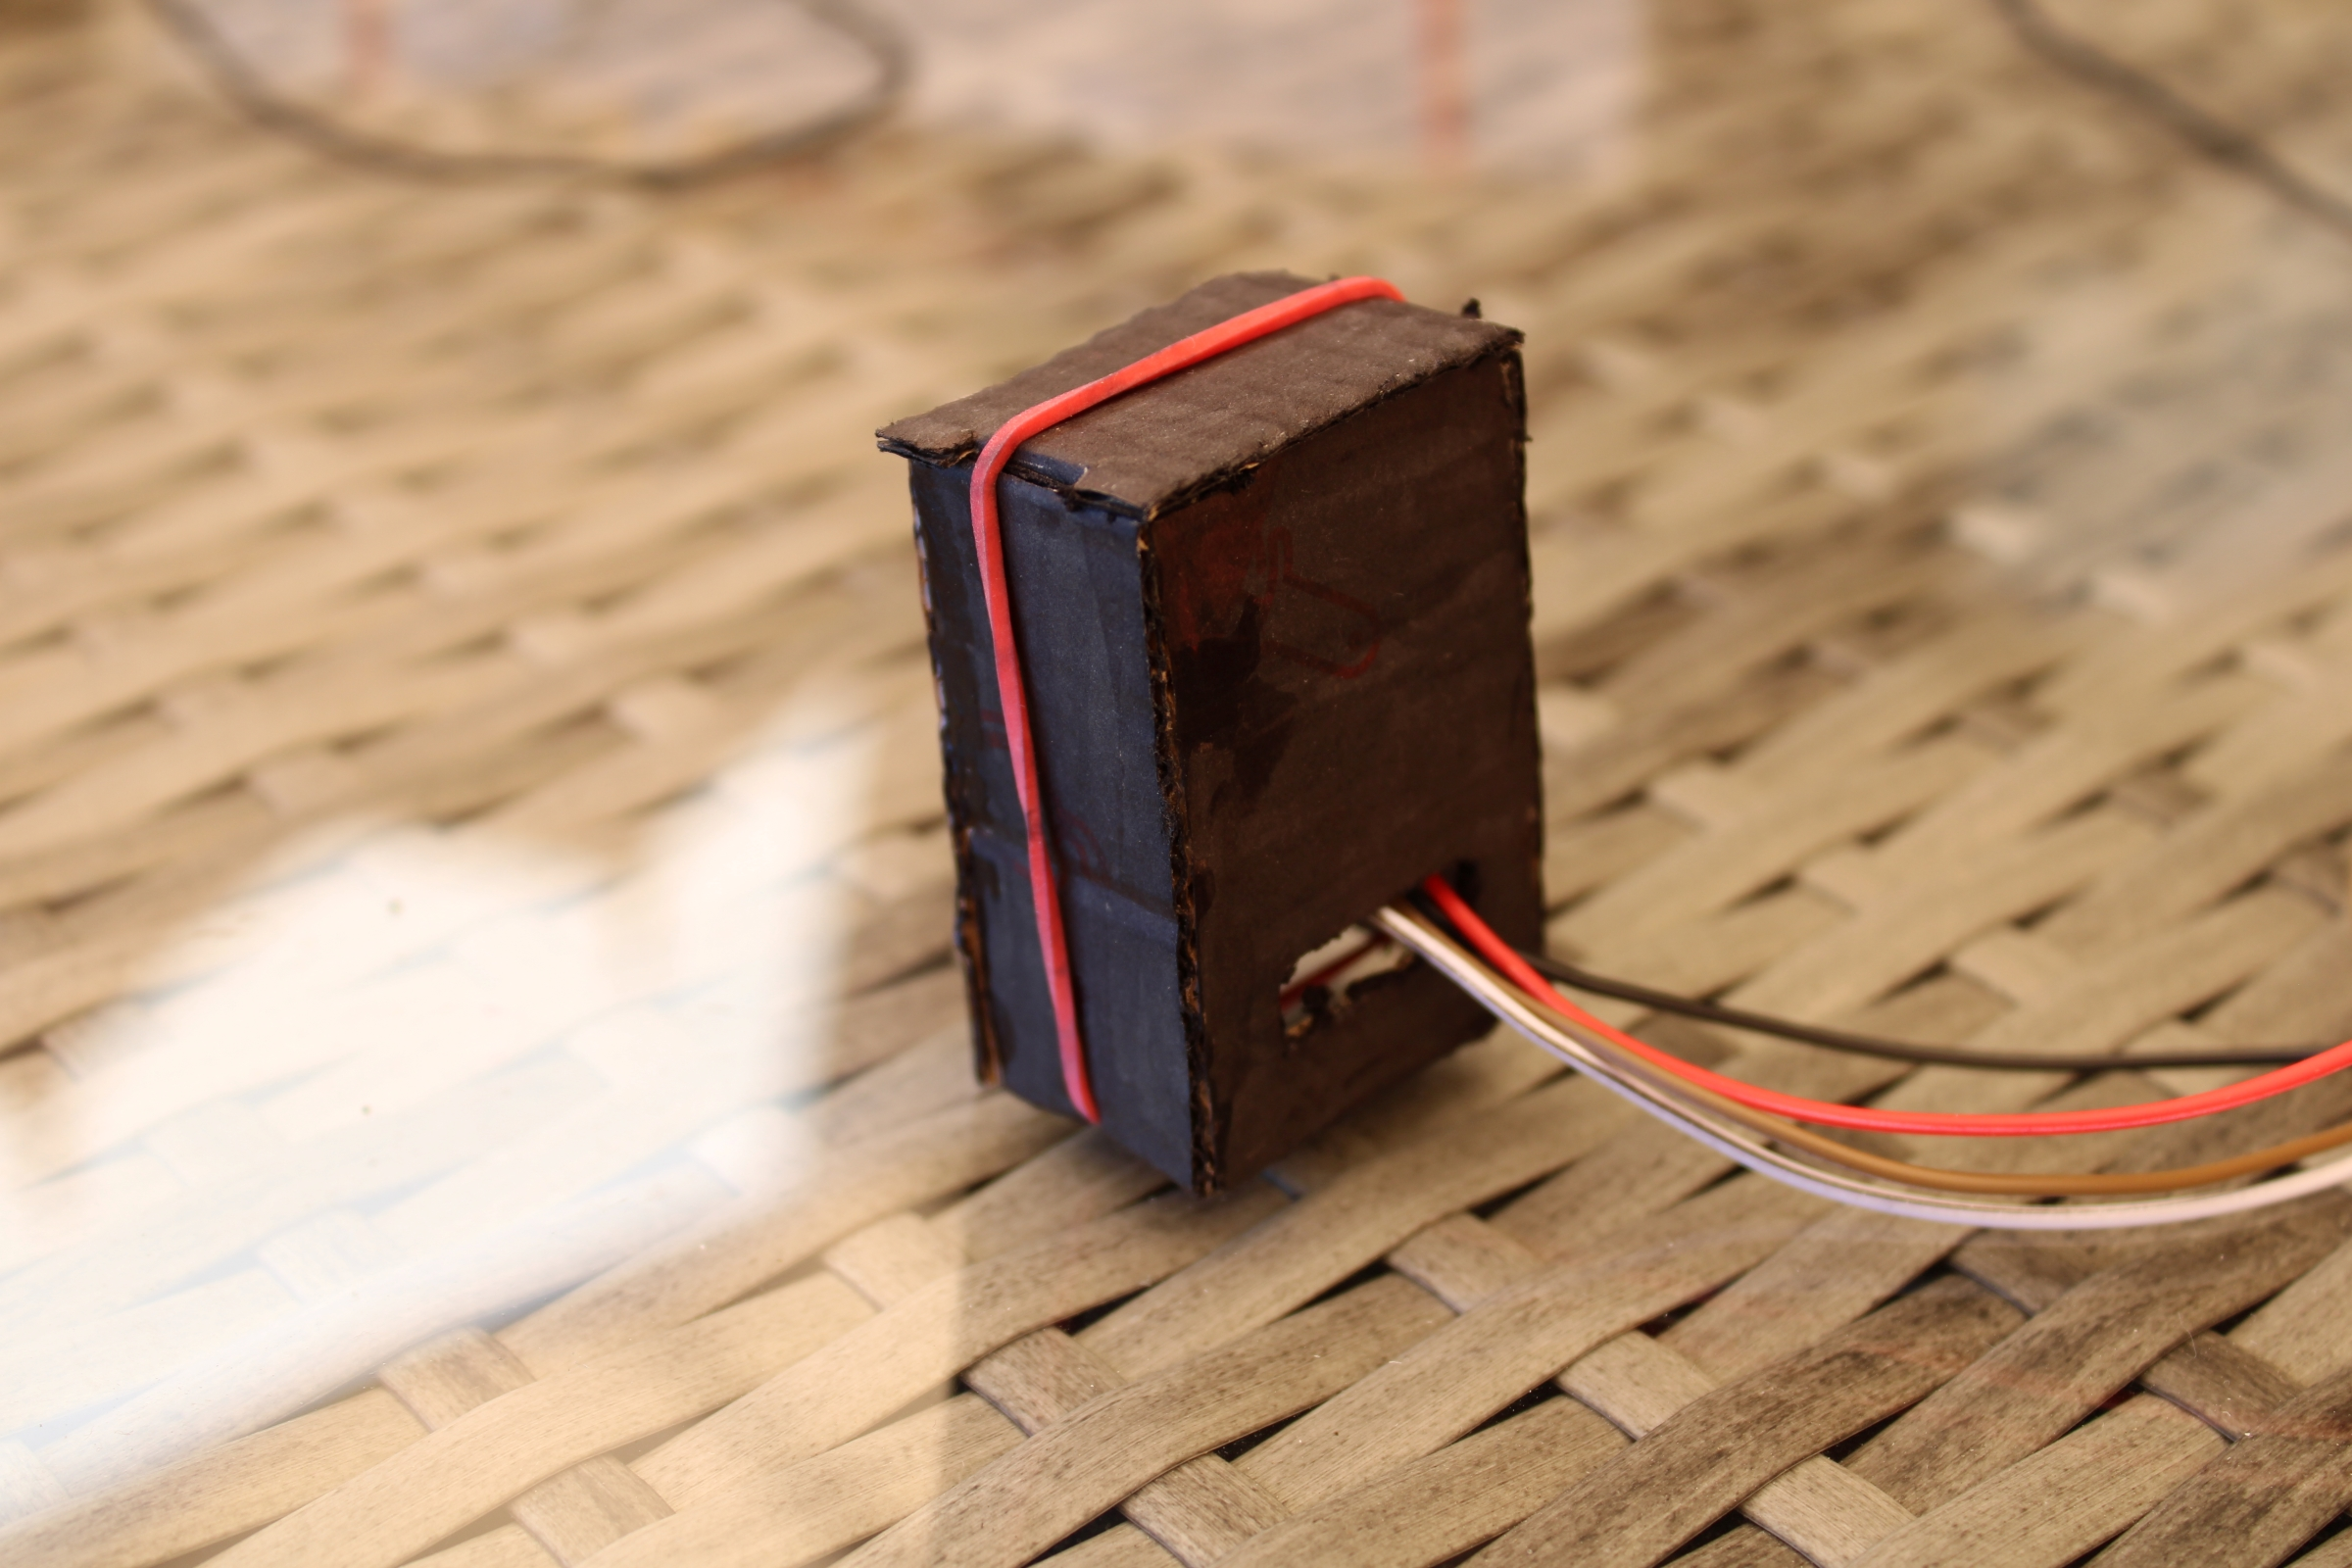
\includegraphics[width=0.4\textwidth]{img/SensorV2_2.jpg}
    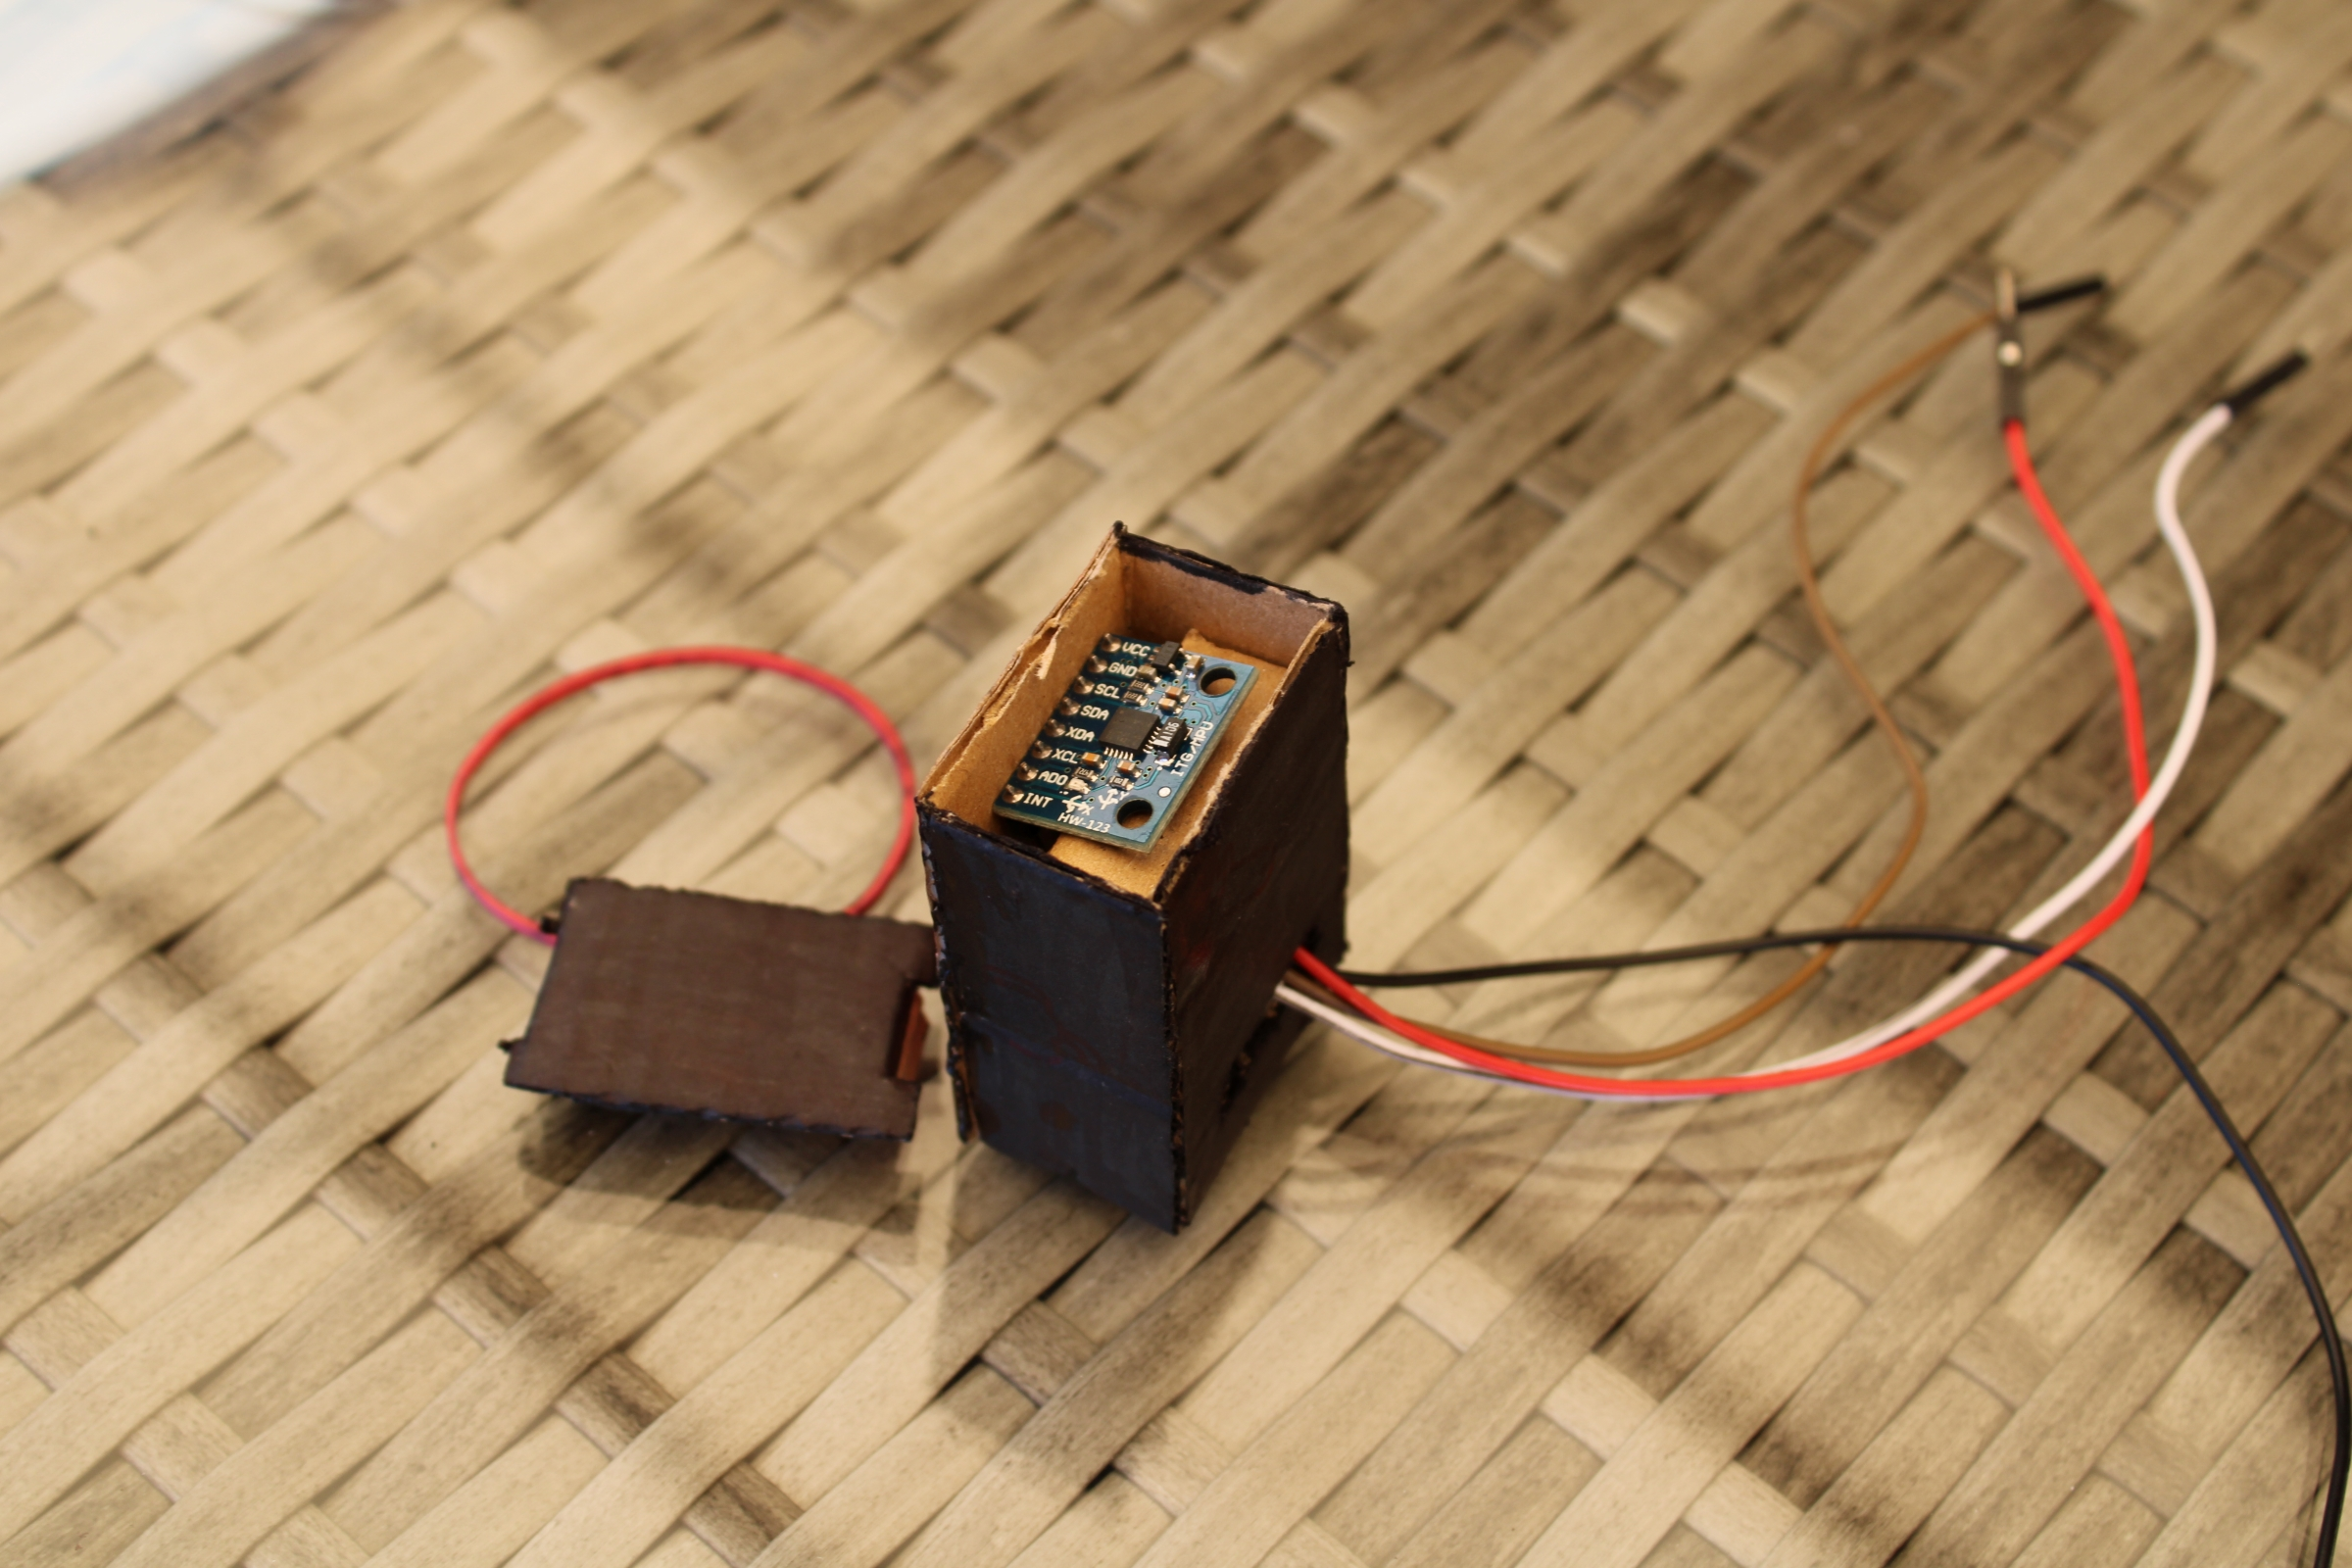
\includegraphics[width=0.4\textwidth]{img/SensorV2_3.jpg}
    \caption{Imágenes del sensor y su base de la segunda versión del prototipo. Fuente Propia.}
    \label{fig:imgDispositivo_V2_sensor} 
\end{figure}

Para más información y demostraciones de los prototipos se recomienda consultar los anexos correspondientes. Además, en el anexo A se han analizado los costes y la viabilidad legal del proyecto.

Por otro lado, se ha diseñado un prototipo de interfaz de una aplicación que facilite la interacción del usuario con el dispositivo y que permite un mejor monitoreo y conocimiento de la postura del usuario. En el prototipo de interfaz se plantea no solo las modificaciones de los ajustes del dispositivo, sino que también la visualización de estadísticas de la postura del usuario y la realización de juegos o ejercicios que se incluirán en la aplicación, para el desarrollo musculoesquelético reforzando aquellos músculos relacionados con la postura y facilitando el aprendizaje muscular de una postura natural correcta. Se puede conocer más información respecto a este prototipo de interfaz en el \textit{Anexo F}.


\section{Discusión.}

En la primera fase se obtiene el resultado que se esperaba, cumple con la función de control postural, pero no se trata de un sensor muy aceptable frente a vibraciones y no es capaz de registrar datos ya que este dispositivo únicamente trabaja como un interruptor en función de la inclinación en la que se encuentre el sensor, es decir, la persona.

Observando y analizando los fallos encontrados en esta primera versión se realizó el segundo prototipo, dónde se empleaba el módulo MPU-6050\cite{MPU6050_1,MPU6050_2}, este prototipo ofrece mayor precisión y posibilita recoger datos. Sin embargo este sensor no está pensado para uso prologado, ya que produce deriva.

Este último problema de deriva se podría solucionar con un sensor algo más complejo pero similar al MPU-6050, el MPU-9250\cite{MPU9250_1,MPU9250_2} que incluye un magnetómetro que soluciona este problema. Este último sensor es el qué se habría pensado para una tercera versión pero que no ha sido posible realizar.

% Discusion 
La realización de este tipo de trabajo no solo ha mejorado el control de distintas herramientas como Arduino, Overleaf o GitHub sino que ha proporcionado la comprensión del proceso completo desde la comunicación de una necesidad real hasta la elaboración de un prototipo pasando por la creación de la idea y la selección de los componentes.

Así mismo, este trabajo sirve como ejemplo de las posibilidades y la importancia que ofrece una visita a una asociación, cómo es la Asociación Parkinson Burgos\cite{ParkinsonBurgos}, dónde se nos ha mostrado el día a día de las personas con esta afectación de la mano de los profesionales, que indicaron necesidades reales y concretas. 

Sin embargo, queda todavía camino que recorrer para obtener un dispositivo de calidad útil. Para conseguir este dispositivo sería interesante trabajar en conjunto con asociaciones o profesionales que evalúen la utilidad del dispositivo. Al formar parte de la primera promoción del grado, es la primera vez que se realiza un TFG de estas características, y no ha sido posible integrarse en un laboratorio en concreto para trabajar en conjunto. Cómo se trata de un trabajo de fin de grado muy amplio, existen todavía varios puntos que reforzar. Con todo ello, espero que este trabajo sirva para conocer limitaciones, dificultades y posibles carencias para el futuro.


\section{Aspectos relevantes.}

Se pueden destacar varios aspectos relevantes del proyecto unos relativos a la creación de la idea y otros a la hora de la creación de los prototipos.

\subsection{Selección del tipo de dispositivo}
Tras identificar las características básicas de la postura y el control postural, se ha realizado un estudio de los dispositivos de control postural y de diagnóstico de alteraciones de la postura para poder recoger las características principales que se quieren incluir en nuestro dispositivo. 

A partir de las distintas opciones estudiadas en el estado del arte, se decidió que el dispositivo objetivo fuese un dispositivo portátil que controlase la postura de una persona según la inclinación de su postura, para ello se iba emplear aprendizaje dinámico basado en biofeedback vibratorio. Este modelo de biofeedback no solo permite controlar la postura sino que también permite la mejora de la misma a largo plazo. Este aprendizaje de biofeedback se basa en que si el dispositivo detecta una mala postura del usuario se envían avisos de vibración o sonoros para que sea accesible a todas las personas ya tengan alguna discapacidad o no. 

Además, se pretende diseñar una aplicación móvil que reúna las características más relevantes de dispositivos existentes y que interaccione con el dispositivo para que el usuario tenga a su disposición los ajustes del dispositivo, sus estadísticas de mejora en su postura, distintos ejercicios que pueda realizar para mejora de su musculatura troncal y por consiguiente su postura.

Asimismo, la idea era avanzar a modo de Kit teniendo un prototipo base e ir añadiendo componentes para evaluar sus posibilidades y personalizar el dispositivo según las necesidades específicas del usuario.

\subsection{Selección de componentes y diferentes versiones}
Una vez clara la idea base del dispositivo que se pretendía crear, se estudiaron las herramientas y componentes disponibles a nuestra disposición y se seleccionó trabajar con Arduino y su placa UNO R3 ya que se ha empleado en algunas asignaturas del grado. Una vez seleccionado el microprocesador se buscaron componentes compatibles con la plataforma.

Seguidamente, se estudiaron varios sensores que podrían ser útiles para el control postural y se seleccionó en primera opción el sensor SW520D debido a su sencillez y bajo precio.

El primer prototipo se realizó empleando el sensor SW520D y una vez se obtuvo el prototipo se analizó su funcionamiento. Sin embargo, para que realizara un correcto control postural era necesario colocar el sensor en un determinado ángulo por lo que sería necesario crear una carcasa donde encaje el sensor en ese ángulo o mantener el dispositivo con algún tipo de control de nivel\footnote{En la figura \ref{fig:imgDispositivo_V1_sensor} se puede ver la carcasa improvisada para realizar el correcto control postural.}. Por otro lado, este primer sensor es muy sensible a vibraciones por lo que no es de gran precisión y no proporciona datos exactos, por ello, se decidió seguir con el siguiente prototipo.

Para el segundo prototipo se decidió emplear el MPU-6050 por su precisión y precio. Este sensor incluye un acelerómetro y un giroscopio que permite conocer en todo momento aceleraciones y rotaciones y, en consecuente, inclinaciones en los distintos ejes. Una vez creado el nuevo prototipo se implementó un programa en el que se incluía el águlo umbral para considerar buena postura y el tiempo de espera para avisar de una postura incorrecta y de esta forma monitorizar la misma. Este prototipo permite recopilar las distintas aceleraciones y rotaciones y por lo tanto estos datos se podrían emplear para realizar distintas estadísticas que se puedan mostrar al usuario.

No obstante, este último prototipo requiere de calibración cada vez que se emplea el dispositivo para poder mantener la buena precisión y, para la calibración el dispositivo no se debe mover y debe estar sobre una superficie plana, por lo que se ha tenido que crear una base de sustentación. Esta base se ha creado con material reciclado de cartón\footnote{En la figura \ref{fig:imgDispositivo_V2_sensor} se puede ver la base de sustentación improvisada para realizar el correcto calibrado y, en consecuencia, el correcto control postural.}.

Asimismo, el módulo MPU-6050 tiene un problema de deriva por lo que no es apto para uso prolongado. Para solucionar este problema se puede emplear el módulo MPU-9250 que sería el sensor una nuestra tercera versión, que no se ha podido realizar por falta de tiempo.




